\documentclass[11pt]{extarticle}
\usepackage{fullpage}
\usepackage[ampersand]{easylist}
\ListProperties(Hide=10, Style*=$\bullet\;\,$, Style2*=$\;\,${\tiny$\blacksquare$}$\;\,$,Space*=1mm,Space2*=0.1mm)

\usepackage{hyperref}
\hypersetup{colorlinks=true,
	linkcolor=black,
	filecolor=black,      
	urlcolor=black}
	
\usepackage{amsmath,amssymb,amsthm,mathtools,mathrsfs}
\newtheorem{thm}{Theorem}[]
\usepackage{bibref}

\usepackage[T1]{fontenc}
\usepackage[sc,osf]{mathpazo}
\usepackage{eulervm}

\usepackage{tikz}
\usetikzlibrary{calc}
\usetikzlibrary{shapes}
\usepackage{pgfplots}
\pgfplotsset{trig format plots=rad}
\usetikzlibrary {3d}
\pgfplotsset{compat=1.18}

\usepackage{multicol}
\setlength{\columnsep}{5mm}
\setlength\columnseprule{.1pt}

\usepackage[most]{tcolorbox}
\tcbuselibrary{skins}
\usepackage[explicit]{titlesec}
\newtcolorbox{secbox}[1][]{enhanced,attach boxed title to top center,drop fuzzy shadow,breakable,colbacktitle=gray,colback=black,colframe=black,
	coltext=white,size=title,title={#1}}
\titleformat{\section}[runin]{\bfseries\LARGE}{}{0pt}{\hfill
	%\begin{secbox}[\thesection]
	%	\centering #1
	%\end{secbox}
	%}
\tcbsidebyside[sidebyside adapt=left,segmentation style=solid,enhanced,size=small]
{%
	\thesection 
}
{%
	#1
}
}
\titleformat{\subsection}[runin]{\bfseries\large}{}{0pt}
{\hfill
%	\begin{secbox}[\thesubsection]
	%		\centering #1
	%	\end{secbox}
\tcbsidebyside[sidebyside adapt=left,segmentation style=solid,enhanced,size=small]
{%
	\thesubsection 
}
{%
	#1
}
}
\titleformat{\subsubsection}[runin]{\bfseries}{}{0pt}
{\hfill
%		\begin{secbox}[\thesubsubsection]
	%			\centering #1
	%		\end{secbox}
\tcbsidebyside[sidebyside adapt=left,segmentation style=solid,enhanced,size=small]
{%
	\thesubsubsection 
}
{%
	#1
}
}

\usepackage{tocloft}

\cftsetindents{section}{0em}{2em}
\cftsetindents{subsection}{0em}{2em}

\renewcommand\cfttoctitlefont{\hfill\Large\bfseries}
\renewcommand\cftaftertoctitle{\hfill\mbox{}}

\setcounter{tocdepth}{2}

\newcommand{\R}{\mathbb{R}}
\newcommand{\C}{\mathbb{C}}
\newcommand{\Na}{\mathbb{N}}
\newcommand{\Z}{\mathbb{Z}}
\newcommand{\Q}{\mathbb{Q}}
\newcommand{\ra}{\rightarrow}
\newcommand{\w}[1]{\text{#1}}
\newcommand{\ck}{.\,.\,}
\newcommand{\sm}[2]{\displaystyle\sum_{#1}^{#2}}
\newcommand{\Uint}[2]{\overline{\int\!}_{#1}^{\;#2}}
\newcommand{\Lint}[2]{\underline{\int\!}_{\;#1}^{\;#2}}
\newcommand{\pfrac}[2]{\frac{\partial#1}{\partial#2}}
\newcommand{\ckfil}{$.\dotfill.$}
\newcommand{\snote}[1]{{\footnotesize(#1)}}
\newcommand{\y}{$\blacksquare\;$}
\newcommand{\smdp}{ \,
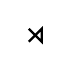
\begin{tikzpicture}
	\draw[thick] (0,0)--(1ex,1ex)--(1ex,0)--(0,1ex);
\end{tikzpicture} 
\,
}
\newcommand{\gen}[1]{\langle #1 \rangle}
\newcommand{\pst}{ \,\rotatebox[origin=c]{90}{$ \gen{||} $} \,}
\newcommand{\tbx}[2][]{
	\begin{tcolorbox}[enhanced,breakable,size=small,colback=black!2!white,title={#1},arc is angular, arc=1.5mm,drop fuzzy shadow]
		#2
	\end{tcolorbox}
}
\newcommand{\tm}{\times}




\author{Yashas.N}
\title{Abstract Algebra: Group Theory.}
\date{}
\begin{document}
\maketitle
\boldmath

\begin{multicols}{2}
\tableofcontents
	\section*{symbols or terms used}
	\tbx{\begin{center}
			$|\ra$ divides i.e. $a|b$ implies $a$ divides $b.$\\
			$(m,n)\ra gcd(m,n)$\\
			$|a|\ra$ order of element in the group or $|G|\ra$ order of the group.\\
			$\forall \ra$ for all. \\
			iff $\ra$ if and only if.\\
			$H\ll G\ra$ $H$ is a subgroup of $G$.\\ 
			$H\trianglelefteq G\ra$ $H$ is a normal subgroup of $G$.\\
			$ \Z,\Q,\R,\C \ra  $ integers, rationals, reals and complex numbers respectively.
		\end{center}
	}
	
	\newpage
	\section{Preliminaries}
	\tbx[ G.C.D ]{ greatest common divisor : $(a,b)=d$ i.e. $gcd(a,b)=d$ if $d|a,d|b$ and if 
		there exist $e$
		such that $e|a,e|b$ then $e|d$ \snote{ here $a,b,d,e \in \Z^+$}
	} 
	\tbx[ L.C.M ]{ $lcm(a,b)=c$ then $a|c,b|c$ and if there exist $e$ such that $a|e,b|e$ then
		$c|e$ \snote{here $a,b,c,e \in \Z^+$}
	} 
	\tbx[ Euclidean algorithm ]{ if $a,b\in \Z^+$ then
		
		\begin{center}
			$a=q_0b+r_0$\\
			$b=q_1r_0+r_1$\\
			$r_0=q_2r_1+r_2$\\
			$\vdots$\\
			$r_{n-2}=q_{n}r_{n-1}+r_n$\\
			$r_{n-1}=q_{n+1} r_n$
		\end{center}
		here $ r_0<b $, $ r_{i+1}<r_i $ and $r_n$ is the $gcd(a,b)$ \snote{i.e. when $ r_{n+1}=0 $}.
	} 
	\tbx{ if we reverse the Euclidean algorithm i.e. write $r_n=r_{n-2}-q_nr_{n-1}$ and use the 
		preceding equation for $r_{n-2},r_{n-1}$ to write $r_n$ in terms of $r_{n-3},r_{n-2}$ and 
		repeating this process we get 
		\begin{center}
			$ax+by=d=(a,b).$
		\end{center}
		for $a,b,x,y,d\in \Z^+$
	} 
	\tbx[Euler's $\varphi$ function]{ $\varphi(n)$ gives the number of relative primes of $n$
		i.e. there are $\varphi(n)$ numbers $<n$ such that their gcd with respect to (w.r.t) $n$ is
		$1.$ Properties and derivation of $\varphi(n)$:
		
			\y  if $p$ is a prime them $\varphi(p)=p-1.$ \\
			\y  $\varphi(p^a)=p^a-p^{a-1}=p^{a-1}(p-1).$ \\
			\y  if $(a,b)=1$ then $\varphi(ab)=\varphi(a)\varphi(b).$ \\
		from preceding points we have
		for  $n=p_1^{s_1}p_2^{s_2}\ck p_k^{s_k}$ ({\footnotesize $p_i$ prime and $s_i\in \Na$ )}
		\begin{align*}
			\varphi (n) & =\varphi(p_1^{s_1}p_2^{s_2}\ck p_k^{s_k}),\\
			& =\varphi (p_1^{s_1}) \varphi (p_2^{s_2}) \ck \varphi (p_k^{s_k}),\\ 		
			& =p_1^{s_1-1}(p_1-1)p_2^{s_2-1}(p_2-1)\\			
			&\qquad \ck p_k^{s_k-1}(p_k-1).
		\end{align*}
	}
	
	\section{Groups}
	\subsection{Definitions}
	
	\tbx[\textbf{Binary operation}]{function $\star : G\times G \ra G$ (for any set $G$) is a
		Binary  operation.
	}
	\tbx[\textbf{Group} ]{$(G,\star)$ : a set $G$ with an binary operation $\star$ on it is a group 
		if :
		
			\y  $\star$ is associative. \\
			\y  Inverse :  
			for every $a\in G\; \exists a^{-1}\in G$ such that $a^{-1}\star a=a\star a^{-1}=e.$
	}
	
	\tbx{ a Group is abelian or commutative if $\star $ is commutative.
		instead of writing $\star$ it is omitted i.e. we write $ab$ instead of $a\star b$
	}
	\tbx{ Order of an element : for $a\in G$ $|a|=n$ is the smallest +ve integer such that $a^n=e.$
		\\ (here $a^n=\overbrace{a\star a \star a \ck\star a}^{n \w{ times }} $)
	}
	\tbx[\textbf{Subgroup} ]{ a subset $S$ of a group $G$ is a subgroup if $S$ is group under same 
		binary operation as $G$ this is denoted by $ S\ll G $.
		
	}
	\tbx[\textbf{Maximal subgroup } ]{ a proper subgroup $ M\ll G $  is maximal in $ G $ iff $ M\ll H\ll G \implies H=G$ i.e. no other proper subgroup of $ G $ contains $ M .$}
	\newcolumn
	
	\subsection{Basic Properties of Groups}
	\tbx{ $a^{-1}$ is unique for every $a$, $(a^{-1})^{-1}=a.$
		$(ab)^{-1}=b^{-1}a^{-1}.$\\
		$ay=b,xa=b$ has a unique solution for every $a,b\in G$ i.e right cancellation and left
		cancellation laws holds in a group.}
	\tbx{ for $a,b\in \Na$ :\\
		$x^ax^b=x^{a+b},(x^{a})^{b}=x^{ab}, (x^a)^{-1}=x^{-a}.$
	}
	\tbx{ if $|x|=n,\, n=st$ then $|x^s|=t$
	}
	\tbx[ \textbf{Cyclic subgroup} ]{ $\gen{x}=\{x^n|n\in \Z^+\}$ forms as subgroup
	}
	\tbx{ if $A,B$ are groups the $A\times B=\{(a,b)|a\in A,b\in B\}$ with component wise group 
		operations forms a group with \\
		$|(a,b)|=lcm(|a|,|b|)$
	}
	\tbx{ $H$ is a subgroup of $G$ ( $H\ll G$) then :
		
			\y   $H$ is closed under group operations and inverses \\
			\y   $ab^{-1}\in H \, \forall a,b\in H$ 
		
	}
	\tbx[Torsion subgroup ]{ if $G$ is an abelian group then $\{g\in G:|g|<\infty\}$ is a subgroup of
		$G$ (if $G$ is an non-abelian infinite group this may not hold )
	}
	\tbx{ if $H,K\ll G$ then :
		
			\y  $H\cap K \ll G$. \\
			\y $H\cup K \ll G$ iff $H\subseteq K$ or $K\subseteq H$.
		
	}
	\section{Homomorphism and Isomorphisms}
	\tbx[\textbf{Homomorphism} ]{ a map $\phi: G\ra H$ for groups $(G,\star),(H,\diamond)$ is 
		a homomorphism if \\ $\phi(a\star b)=\phi(a)\diamond\phi(b)\; \forall a,b\in G$ 
	}
	\tbx[\textbf{Isomorphisms} ]{ a map between two groups $\phi$ is isomorphism if it is homomorphism
		and bijective (one-one and onto).}
	\subsection{Basic Properties of group related to homo and isomorphisms}
	\tbx{ if $\phi : G\ra H$ is homomorphism then
		
			\y  $\phi (x^n)=\phi (x)^n\; \forall x\in G,\forall n\in \Z$ \\
			\y  kernel( $\phi$) $=ker(\phi)\\ 
			=\{x|\phi(x)=e_H(\w{ identity of }H)\}$ is subgroup of $G$\\
			\y  image under $\phi$ i.e. $\phi (G)$ is a subgroup of $H$ \\
			\y  $\phi$ is injective iff $ker(\phi)=\{e_G\}$ 
	}
	
	\tbx{ if $\phi: G \ra H$ is isomorphism then 
		
			\y  $|G|=|H|$ \\
			\y  $G$ is abelian iff $H$ is abelian \\
			\y  $|x|=|\phi (x)|\; \forall x\in G$ 
		}
	
	\tbx{ The map $\psi : g\ra g^{-1}$ in $G$ is homomorphism (isomorphism to be specific) iff $G$ is abelian.
\snote{use $ \psi((ab)^{-1})= ab ,\; \psi(b^{-1}a^{-1})=ba$}	}
	\tbx{ The map $\psi : g\ra g^2$ in $G$ is homomorphism iff $G$ is abelian.
	}
	\tbx{ if $A$ is abelian then the map $\psi : a\ra a^k$ is a homomorphism.}
	\section{Automorphism $Aut(\;)$}
	\tbx{ $Aut(G)$ is the set of all isomorphism of a group $G$ onto itself.\\
		$Aut(G)$ forms a group under function composition.
		
	}
	\tbx{ if there exists an Automorphism $\phi$ of $G$ such that $\sigma(g)=g \iff g=1$ (i.e. no fixed points ) and $\sigma^2=I$ 
		(Identity) then $G$ is abelian.
	}
	\tbx{ if $A,B$ are groups then $A\times B \cong B\times A$ (isomorphic) 
		(use isomorphic map $\phi :A\times B \ra B \times A $ by $(a,b)\ra (b,a)$).  }
	
	
	\section{Group Actions}
	\tbx{
		Importance is given to group actions as a set `acting' on another set is the major recurring theme not
		only in Group Theory but whole of Mathematics, also plays a major role in proofs as it gives 
		lot of information about structures of `objects' in Mathematics.}
	
	\tbx{A Group Action on of a Group $G$ a set $A$ is a map from $G\times A \ra A$ ( $g.a$ for 
		$g\in G,a\in A$) satisfying the following properties $\forall a\in A, g_1,g_2\in G$
		
			\y  $g_1.(g_2.a)=(g_1 g_2).a$ (here $g_1g_2$ is the group $G$ operation on its members $g_1,g_2$ \\
			\y  $1.a=a$ ( $1$ is identity in $G$) 
		
		Note : if $g$ is fixed then we see that $g.a$ for varying  $a\in A$ acts as a map 
		$\sigma_g:A\ra A$ and from that fact that $g\in G$ (group) we have $g^{-1}\in G$ and 
		$(g^{-1}g).a=(gg^{-1}).a=1.a=a$ thus this map has a left and right inverse so $\sigma_g$ is
		bijection map in $A$
	}
	\tbx{Immediate consequence of the preceding point is that group action of $G$ on $A$ is nothing but 
		a set of permutations (elements of $S_A$ symmetric group in $A$) $\sigma_g:A\ra A$ given by
		$\sigma_g(a)=g.a$ 
	}
	\tbx{from preceding point and group actions obey a kind of group properties ( $G$ )  we get :
		\begin{center}
			the map $g\ra \sigma_g \in S_A$ is a \textbf{Homomorphism}\\
			i.e. Group actions can be summarized as a homomorphism $\phi : G\ra S_A$. 
		\end{center}
	}
	\tbx[\textbf{Faithful }]{a group action is faithful if distinct elements in $G$ 
		produce distinct permutations of $A$ i.e. the homomorphic map $\phi$ of the group action 
		is injective.
	}
	\tbx[\textbf{Kernel of action}]{ kernel of a group action is the set $\{g\in G|g.a=a\, \forall a\in A\}$.
	}
	\tbx{a Group action is faithful iff its kernel $={1}$.
	}
	\tbx[\textbf{Stabiliser} ]{for $a\in A$ Stabiliser of $a$ (for group action $G$ on $A$) is set 
		$G_a=\{ g\in G|g.a=a\}$
		
			\y  Kernel of the group action is contained in every Stabiliser. \\
			\y  Define a relation $\sim$ on set $A$ with group action $G$ on $A$ as : \\
			\y  $a\sim b$ iff $a=g.b$ for $g\in G$ \\
			\y  then $\sim $ is equivalence relation  
		
	}
	\tbx[\textbf{Orbit}]{ orbit of $x\in A$ under action of $G$ is the equivalence class of $x$ under the preceding
		relation $\sim $ i.e $ \mathcal{O}_x=\{y\in A |x=gy \w{ for } y\in A,g\in G \}$
	}
	\tbx{Clearly Kernel of an group action (of $G$) and Stabiliser of an element are subgroups of $G$.
	}
	\tbx{Number of elements in the orbit or equivalence class of $a$ :
		\begin{center}
			$| \mathcal{O}_a|=|G:G_a|.$
		\end{center}
		{\footnotesize (use bijective map from $C_a=\{g.a|g\in G\}\ra \{gG_a\}$ by $b=g.a\ra gG_a$. )}
	}
	\tbx[ \textbf{ Transitive }]{A group action of $ G $ on $ A $ is transitive if there exist only one orbit for 
		the action i.e. $ \mathcal{ O}_a=A \forall a \in G .$}
	\subsection{ Major Group Actions}
	\subsubsection{Conjugation}
	
	\tbx{define a group action (conjugation) $:$ of $G$ to its power set $P(G)$ by 
		\begin{center}
			$g:B\ra gBg^{-1}=\{gbg^{-1}|b\in B\}.$ 
		\end{center} for $B\subseteq G,g\in G$
	}
	\tbx[\textbf{Centralizer} ]{
		\y centralizer of an element $a\in G$ in $G$ $C_G(a)$ is the Stabiliser of $a$ under 
		conjugation i.e. $C_G(a)= \mathcal{O}_{\{a\}}=\{g\in G|gag^{-1}=a\}$ i.e. all the elements that 
		commute with $a$. \\
		\y centralizer of a  $A\subset G$ in $G$ $C_G(A)$ is the intersection of all the 
		centralizer of elements of $A$ in $G$ i.e. $C_G(A)=\underset{a\in A}{\cap} \mathcal{O}_{\{a\}}
		\\= \{ g\in G|gag^{-1}=a \forall a\in A\}$ i.e. all the elements of $G$ that commute with every 
		element of $A$.
	}
	\tbx[Normalizer]{ Normalizer  of $A\subset G$ in $G$ $N_G(A)$ is the Stabiliser of $A$ under conjugation
		i.e. $N_G(A)=G_a=\{g\in G|gAg^{-1}=A\}$
	}
	\tbx[\textbf{Center}]{center of $G$ denoted by $Z(G)$ is the kernel of conjugation i.e. elements of $G$ that commute 
		with every element of $G.$
	}
	\tbx{Basic properties induced by conjugation :
		
			\y  $C_G(Z(G))=N_G(Z(G))=G.$ \\
			\y   $Z(G)\ll C_G(A)\ll N_G(A)\ll G.$ for any $A\subset G$ \\
			\y   if $A\subset B$ then $C_G(B)\ll C_G(A).$ 
		
	}
	\tbx[\textbf{ Normal } ]{$ N\ll G $ is said to be normal in $ G $ ( $ N\trianglelefteq G $) if $ N_G(N)=G $
		i.e. $ gNg^{-1}=N\; \forall g \in G $
	}
	\tbx{if $ H\trianglelefteq G$,  $ K\trianglelefteq G$ then $ H\cap K \trianglelefteq G $
	}
	\tbx{now as $ |\mathcal{ O }_a|=|G:G_a| $ we get :
		\begin{center}
			number of conjugates of a subset $ S $ of $ G $ is\\
			$ |\{gSg^{-1}\}|=|G:N_G(S) |.$\\
			in particular the number of conjugates of $ a\in G $ \\
			$  |\{gag^{-1}\}|=|G:C_G(a)|.$
		\end{center}
	}
	\tbx{two elements $ a,b\in G $ are conjugates in $ G $ if $ a =gbg^{-1} $ for some $ g\in G .$
	}
	\tbx{we can form a group action of $ G $ acting on itself by conjugation i.e. $ g:a=gag^{-1} $ for $ a,g\in G $ then 
		this forms an equivalence relation defined by preceding point in $ G $  the equivalence classes of this relation
		is called \\ \textbf{conjugacy classes }  of $ G .$  
	}
	\tbx{\y if $ a $ and $ b $ belong to same conjugacy class i.e. $ a=gbg^{-1} $ then $ |a|=|b| $ \\
		\y if $ 2||G| $ and $ a\in G $ then $ a^2\notin   $ conjugacy class of $ a $ \\
		\y if $ G $ is of odd order then for non identity element $ x \in G$ is not a conjugate of $ x^{-1} $ \snote{use : $ x\sim x^{-1} $ then as $ 2\not| |G| $ we have $ x\neq x^{-1} $ so similarly we have $ x\sim y\implies y\sim y^{-1} $ so conjugacy class of $ x $ has an even order.}
	}
	\tbx{if $ H\trianglelefteq G $ and $ H $ is non trivial (i.e. $ H\neq \{1\}, H\neq G $) then for a conjugacy class $ \mathcal{ C } $ of $ G $ : $ \mathcal{ C }\subset H $ or $ \mathcal{ C }\cap H =\emptyset .$}
	
	\subsubsection{Left (right) multiplication}
	\tbx[\textbf{Cosets} ]{ a Group can act on its subgroup by left multiplication to produce sets called cosets i.e.
		for $ H\ll G $ define $ g.H=gH=\{gh|h\in H\} $ in fact group action can only be produced (well 
		defined) if $ G $ acts on the set of cosets (left) of $ H\ll G $
	}
	\tbx{ Properties of Left Multiplication : if $ G $ acts on cosets of $ H\ll G $ in $ G $ by left multiplication then
		
			\y  Left Multiplication is Transitive  \\
			\y  Stabiliser of $ 1H = G_H=H$ \\
			\y   Kernel of this action is $ \{g|g.xH=xH \forall x\in G\}=\underset{x\in G}{\cap}xHx^{-1} $ which is the largest normal  
			subgroup of $ G $ contained in $ H. $
		
	}
	\tbx{now if we take $ H={1}\ll G $ then we get Cayley's Theorem (as one can intrepret this 
		group actions as homomorphism from $ G\ra S_G $)
	}
	\tbx{number of left cosets of $ A\ll G $ is called \textbf{index} of $ A $ in $ G $ and is denoted by $ |G:A| $ 
	}
	\tbx{if $ G $ is finite group then for $ H\ll G $ \\$ |G: H|= \frac{ |G| }{|H|}$ (by Lagrange's Theorem).
	}
	\tbx{if $ H,K \ll G $ of finite index in $ G $ (possibly an infinite group ) i.e. $ |G:H|=m,\; |G:K|=n $ then 
		\begin{center}
			$ lcm(m,n)\leq |G:H\cap K| \leq mn .$
		\end{center} (in particular if $ (mn)=1 $ then $ |G:H\cap K|=mn $.)
	}
	\tbx{if $ H\ll K\ll G $ then
		\begin{center}
			$ |G:H|=|G:K| \,|K:H| .$
	\end{center}}
	
	\section{Quotient Groups}
	
	\tbx{Fiber : another word for preimage. It can be imagined as a comparison of a cloth to a function
		and the therads or fibers weaive to make up the cloth i.e. the preimages make up the functions
		at particular value.
	}
	\tbx{for any $ N \ll G $ (group) and $ g\in G $ we have \\
		$ gN=\{gn|n\in N\} $ is called a left coset of $ N $ in $ G $ and $ Ng=\{ng|n\in N\} $ the right    coset.
	}
	\tbx{for any homomorphisms $ \phi : G\ra H $ between two groups with Kernel $ K $ then
		 \tbx[\textbf{ Quotient Group } ]{let $ G/K $ be the set containing the fibers preceding $ a\in H $ 
				i.e. $ G/K = \{X\subset G|\phi^{-1}(a)=X\}.$ }
			\y  left cosets of $ K $ in $ G $ are equal to right cosets of $ K $ in $ G $ i.e. $ gK=Kg \,  
			\forall g\in G$ i.e. $ K $ is normal in $ G $\\
			\y  Members of $ G/K $ are only the left cosets (or right cosets) of $ K $ in $ G $\\ 
			i.e. if $ X\in G/K $ then $ X=\phi^{-1}(a)= uK$ for some $ u\in G $ i.e. if $ u\in X $ then 
			$ X=\{uk|k\in K\} $ only.
			}
	\tbx{Now for any $ N\ll G $ : \\
			\y  The set of left cosets (right) of $ N $ in $ G $ partition $ G $ and 
			$ uN=nN $ iff $ v^{-1}u \in N $.\\
			\y  The operations $ uN.vN=(uv)N $ is well defined iff $ gng^{-1}\in N\, \forall g\in G, n\in N $ 
			i.e. iff $ N $ is normal in $ G .$ By this opeartions (if well defined) the cosets of 
			$ N $ in $ G $ : $ \{gN\} $ forms a group.
		
	}
	\tbx{Now if $ N \trianglelefteq G $ ({\footnotesize $ N $ normal in $ G $  )} iff :\\
			\y  $ gN=Ng \; \forall g \in G$  \\
			\y   $ N $ is a kernel of some homomorphism from $ G $, namely the natural projection homomorphism 
			$ G $ onto $ G/N $ i.e. $ \pi :G\ra G/N $ given by $ \pi (g)\ra gN $ has the kernel $ N .$
		
	}
	\tbx{\textbf{ Quotient group of Cyclic groups are cyclic. }
	}
	\tbx{if $ B\ll A $ an abelian group then $ A/B $ is abelian.
	}
	\tbx{if $ G/Z(G) $ is cyclic then $ G $ is abelian 
	}
	\tbx{for $ N\trianglelefteq G $ $ xN, yN $ commute iff $ x^{-1}y^{-1}xy \in N $
	}
	\tbx{Commutator subgroup of G : $ N= \langle x^{-1}y^{-1}xy|x,y\in G \rangle $ (set generated by 
		these elements) then $ N $ is normal in $ G $ and $ G/N $ is abelian.
	}
	\tbx{if we define $ HK=\{hk|h\in H,k\in K\} $ for some $ H,K \ll G $ then
		
			\y  $ HK \ll G$ iff $ HK=KH .$\\ 
			in particular if $ H \ll N_G(K) $ then $ HK $ is a subgroup.\\
			\y  $ |HK|=\frac{ |H||K| }{|H\cap K|} .$ 
	
	}
	\tbx{ if $ H\trianglelefteq G $ and is of prime index i.e. $ |G:H|=p $ then for any $ K\ll G $ either \\
	\y $ K\ll H $ or \\
	\y $ G=HK $ and $ |K:H\cap K|=p$ \\
	\snote{use $ G/H\cong Z_p $ so if $ g\in K $  and $ g\notin H $ then $ gH $ generates $ G/H $ so every element of $ G $ is of form $ g^ih_i $ for some $ h_i\in H $ and for index use $ 2^{nd} $ isomorphism theorem }}
	\tbx{ if $ A\trianglelefteq G $ and $ B\trianglelefteq H $ then $ A\tm B \trianglelefteq G\tm H $  and 
	$ (G\tm H)/ (A\tm B)\cong (G/A) \tm (H/B)$ 
	 }
	 \tbx{if $ M,N \trianglelefteq G $ are such that $ G=MN $ then $ G/(M\cap N)\cong (G/M)\tm (G/N) $  }
	\section{Cyclic Groups and order}
	
	\tbx{a Group is cyclic if it is generated by a single element i.e. $G=\{x^n|n\in \Z \}
		=\langle x\rangle $
	}
	\tbx{if $H=\langle x\rangle $ then
		
			\y  $|H|=|x|$ \\
			\y   if $|x|=n<\infty$ then $H=\{1,x,x^2,\ck,x^{n-1}\}.$ \\
			\y   if $|x|=\infty$ and if $ a,b\in \Z$ are such that $a\neq b$ then $x^a\neq x^b.$  \\
			\y if $ |x|=\infty $ then for $ a,b\in Z $ $ \gen{x^a}=\gen{x^b} $ iff $ a=\pm b .$ 
		
	}
	\tbx{if for $m,n\in \Z$, $x\in G$ (group) such that $x^n=1,\, x^m=1$ then for $d=(m,n)$ 
		we have $x^d=1.$ and in particular $x^m=1\implies m||x|.$
	}
	\tbx{Any two cyclic groups of same finite order are isomorphic and a cyclic group of infinite order
		is isomorphic to $\Z.$ So cyclic group of order $ n $ can be considered as $ Z_n=\Z/n\Z $.
	}
	\tbx{for $x\in G$ (group) we have
		
			\y  if $|x|=\infty$ then $|x^a|=\infty$ for every $a\in \Z -\{0\}$ \\
			\y  if $|x|=n<\infty$ then  
			\begin{center}
				$|x^a|= \frac{n}{(n,a)}.$
			\end{center}
		
	}
	\tbx{for $H=\langle x \rangle $ :
		
			\y  if $|x|=\infty$ then $H=\langle x^a \rangle$ iff $a=\pm 1$ \\
			\y   if $|x|=n<\infty$ then $H=\langle x^a \rangle$ iff $(n,a)=1$ \\ 
			so the number of generators of $H$ is $\varphi (n).$\\
			\y   Every subgroup of $H$ is cyclic i.e. if $K \ll H$ then $K=\langle x^k \rangle$ \\ 
			where $k$ is the smallest +ve integer such that $x^k\in K$\\
			\y   Clearly every subgroup of finite cyclic group is unique of the given order i.e. for a group $ G $ if there exist more than one subgroup for a given order then $ G $ is not cyclic \\
			\y   if $|H|=n< \infty $ the for each +ve integer $a$ dividing $n$ there exists a unique subgroup 
			of $H$ of order $a$ i.e. $ \langle x^d \rangle $ for $d=n/a$ is a unique subgroup of order $a$
			in $H.$\\
			\y   from preceding point and as $ \langle x^m \rangle = \langle x^{(m,n)} \rangle $ we get the  
			subgroups of $ H $ corresponds bijectively to divisor of $ n $ where $ |H|=n<\infty $.
		
	}
	\tbx{if $ |x|=n, |y|=m $ for $ x,y \in G $ and if $ x,y$ commute then $ |xy|=lcm(n,m). $
	}
	\tbx{every Automorphism $ \sigma_a $ of $ H= \langle x \rangle $ can be characterised by 
		$ \sigma_a(x)=x^a $ for some $ (n,a)=1 $ from this we get 
		\begin{center}
			$ Aut(Z/nZ)\cong (Z/nZ)^* .$
	\end{center} }
\tbx{\y Every Group is union of its cyclic groups \snote{as $ a\in G\implies \gen{a}\ll G $ so $ G=\underset{a\in G}{\cup}
		\gen{a} $ .} \\
	\y So if $ |G| $ is infinite then it at-least has infinite subgroups.}
		\section{Direct product} 
	\tbx{if $ G_1, G_2 ,\ck , G_n $ are groups with operations $ \star_1, \star_2,\ck , \star_n $ respectively then direct product $ G= G_1\times G_2 \times \ck \times G_n =\{(g_1,g_2,\ck, g_n)|g_i\in G_i\}$ with operation $ \star  $ such that $ (g_1,g_2,\ck, g_n) \star (h_1,h_2,\ck, h_n) =(g_1\star_1 h_2,g_2 \star_2 h_2,\ck, g_n \star_n h_n)$}
	\tbx{ let $ G $ be a direct product as in preceding point then 
		for $ (G,\star) $ :\\
		\y  $ G $ is group of order $ |G_1||G_2|\ck |G_n| $ (if any $ G_i $ is infinite the so is $ G $) \\
		\y  $ G_i \cong \{(1,\ck, g_i,\ck ,1)|g_i\in G_i\} $ this subset is a subgroup of $ G $ \snote{note $ g_i $ is in $ i $th position and $ 1 $ in other positions are identities of respective groups}  \\
		\y  for fixed $ i $ $\pi_i : G \ra G_i  $ by $ \pi_i((g_1,\ck,g_i\ck ,g_n))=g_i $ is a surjective homomorphism such that  
		$ Ker\,\pi =\{(g_1,\ck ,g_{i-1},1,g_{i+1}\ck ,g_n)\} \cong G_1\times \ck \times G_{i-1}\times G_{i+1}\times \ck \times G_n $ \snote{here $ 1 $ is in the $ i $th position.}\\
		\y  if $ x\in G_i $,$ y\in G_j $,$ i\neq j $ if $ \dot{x} =(1,\ck, x\ck ,1)$ \snote{for $ x $ in $ i $th position} and 
		$ \dot{y} =(1,\ck, y\ck ,1)$ \snote{for $ y $ in $ j $th position} then $ \dot{x}\dot{y}=\dot{y}\dot{x} $ i.e. they commute.\\
		\y  $ Z(G_1\times G_2 \times \ck \times G_n ) = Z(G_1)\times Z(G_2 )\times \ck \times Z(G_n )$ i.e. 
		center of $ G $ is the direct product of centers of its products.\\
		\y  if $ \pi \in S_n $ then:\\ 
		$ G_1\times G_2 \times \ck \times G_n \cong G_{\pi(1)}\times G_{\pi(2)} \times \ck \times G_{\pi(n)}  $ i.e the order in the products of direct product doesn't make any difference \\
		\y  if $ I \subset \{1,2,\ck , n\} $,$ J= \{1,2,\ck , n\} -I$, $ G_I \ll G$ is isomorphic  to direct product of $ G_i \w{ for }i\in I$ and \\
		$ G_J \ll G$ is isomorphic to direct product of $ G_j \w{ for }j\in J$ then \\
		$ G_I $ is normal in $ G .$\\
		$ G/G_I\cong G_J.$\\
		$G \cong G_I \times G_J .$
	}
	\tbx[\textbf{Recognition Theorem of Direct product} ]{ If $ H,K \trianglelefteq G $ are such that $ H\cap K =\emptyset$ then 
		\begin{center}
			$ HK\cong H \times K .$
		\end{center} \snote{use fact that there $ |H\cap K| $number of ways of writing elements each element of $ HK .$}}
	\section{Generated subgroups and groups}
	\tbx{ 
		\y for any subset $ A\subseteq G $ define subgroup generated by 
		$ A=\gen{A}=\underset{\substack{A\subseteq H \\ H\ll G}}{\cap} H $  \\
		\y if $ A=\{a_1,a_2,\ck a_n\}  $ then 
		\\$ \gen{A}=\{a_1^{i_1}a_2^{i_2}\ck a_k^{i_n} | a_j \in A, i_l =\pm 1, k\in \Z^+\}$
		\snote{note: $ a_i $ can be equal to $ a_{i+1} $ and so on to give more powers of an element.}\\
		\y if $ G $ is abelian and $ A=\{a_1,a_2,\ck a_n\}  $ then 
		$ \gen{A}=\{a_1^{i_1}a_2^{i_2}\ck a_k^{i_n} |i_j \in Z\} $ }
	\tbx[Finitely Generated Groups]{
		\y A group $ G $ is finitely generated if there exist a finite subset of $ A $ of $ G $ such that $ G=\gen{A} $ \\
		\y every finite subgroup of finitely generated group is finitely generate.
	}
	\section{Simple and solvable Groups}
	
	\tbx[\textbf{Simple Group} ]{ group $ G $ is simple iff the only normal subgroups of $ G $ are trivial subgroups (i.e. $ \{1\} , G$)
	}
	\tbx[\textbf{Composition series}]{Composition series of a group for a group $ G $ is the set inclusion or  a Chain (w.r.t ordering of subgroups) given by
		\begin{center}
			$ \{1\} \trianglelefteq N_0\trianglelefteq N_1\trianglelefteq \ck \trianglelefteq N_{k-1}\trianglelefteq N_k =G.$ 
			\end{center}
			where $ N_{i+1}/N_i $ is a simple group and\\
			$ N_i $ are called composition factors.
	 (note this doesn't mean all $ N_i \trianglelefteq G $ 
		as $ H \trianglelefteq K \trianglelefteq G  $ doesn't imply $ H \trianglelefteq G$ .)
	}
	\tbx{every Group has a composition series and if for same group $ G $ 
		\begin{center}
			$ \{1\} \trianglelefteq N_0\trianglelefteq N_1\trianglelefteq \ck \trianglelefteq N_{k-1}\trianglelefteq N_k =G.$ \\
			$ \{1\} \trianglelefteq M_0\trianglelefteq M_1\trianglelefteq \ck \trianglelefteq M_{s-1}\trianglelefteq M_s =G.$ 
		\end{center}  then $ k=s $ and $ M_{\pi (i)}/M_{\pi(i)-1} \cong N_i/N_{i-1}$ for some permutation $ \pi \in S_k .$
	}
	\tbx{if $ G $ is an abelian simple group then $ G \cong Z_p $ for some $ p $ prime \snote{true even if $ G $ is infinite.} \\
	\snote{ use the fact that every subgroup of abelian group is normal and cauchys theorem.}}
	\tbx[\textbf{Holders Program }]{	\footnotesize
		
		
			\y  Classify all finite simple groups \\
			\y   Find all ways of combining simple groups to form other groups \\
			\y  Classifying all finite simple groups  has been completes in 1970 took more than 5000 Journal pages and a 100 years. Which says that : \\ 
			There is a list of 18 infinite families of simple groups and 26 simple groups not belonging here (sporadic groups)
			such that every finite simple group is isomorphic to  	one of these groups. (for eg $ \{Z_p|p \w{ is a prime}\} $ is one of the infinite families.)
		
	}
	
	
	\tbx[\textbf{Solvable Groups} ]{a group $ G $ is solvable if there is chain of subgroups \\
		$ \{1\} \trianglelefteq G_0\trianglelefteq G_1\trianglelefteq \ck \trianglelefteq G_{s-1}\trianglelefteq G_s =G.$ \\
		such that $ G_{i+1}/G_i $ is abelian.
	}
	\tbx{if $ N(\trianglelefteq G )$ and $ G/N $ are solvable then $ G $ is solvable  
	}
	\tbx{$G $ is finite solvable group with solvable chain 
		$ \{1\} \trianglelefteq H_0\trianglelefteq H_1\trianglelefteq H_{2} \trianglelefteq \ck \trianglelefteq H_s =H.$  iff : \\
		\y  $ H_{i+1}/H_i $ \textbf{is cyclic} 
		\\ \snote{ use argument that $ H_{i+1}/H_{i} $ is simple abelian group as $  
				H_{i}$ is maximal normal subgroup of $ H_{i+1} $.}\\
		\y   all composition factors of $ G $ are of prime order. 
	}
	\tbx{if $ G $ is a finite group in which every proper subgroup is abelian then $ G $ is solvable.}
	\newcolumn
	
	\section{Major Theorems and consequences}
	\subsection{Lagrange's theorem}
	\tbx[Theorem]{if $ G $ is a finite group and $ H $ is a subgroup of $ G $ 
		then :
		
			\y  order of $ H $ divides order of $ G $ \\
			\y   and the number of left cosets (right) of $ H $ in $ G $ i.e index of $ H $ in $ G $  
		\[=|G:H|= \frac{ |G|}{ |H| } .\]
			(can be easily derived by coset theory or respective group action theory)
		
	}
	
	\tbx[Consequences of Lagrange's Theorem :]{
		
			\y  if $ H,K\ll G $ finite group such that $ |H|=n,|K|=m $, and $ (m,n)=1 $ then $  H\cap K=\{1\}.$ \\
			\y  if order of group $ G $ is a prime ( $ p $) then $ G $ is cyclic ($ G\cong \Z/p\Z $) \\
			\y  Fermats little theorem : if $ p $ is a prime then $ a^p\equiv a\pmod{p} \; \forall a\in \Z$. \\
			(apply Lagrange's theorem on $ (\Z/p\Z)^* $
			\y  Euler Theorem (generalized Fermats little theorem) : $ a^{\varphi(n)}\equiv 1\pmod{n} $ for  \\
			every $ (a,n)=1 .$  
			(apply Lagrange's theorem on $ (\Z/n\Z)^* $
		
	}
	\subsection{Isomorphism Theorems}
	\tbx[First Isomorphism Theorem (\textbf{fundamental})  ]{if $ \phi : G\ra H $ is homomorphism 
		of groups then $ G/ker\phi \cong \phi(G) $ (easy direct proof)
	}
	\tbx[Second Isomorphism Theorem (\textbf{diamond}) ]{ for a group $ G $ with subgroups $ A,B $ 
		such that $ A\ll N_G(B) $ then $ AB\ll G,\; B\trianglelefteq AB, \; A\cap B\trianglelefteq A $ 
		and $ AB/B\cong A/A\cap B $.(use homomorphism $ \phi : A\ra AB/B $ by $ \phi(a)=aB $)
		lattice diagram :}
	
	\begin{center}
		
		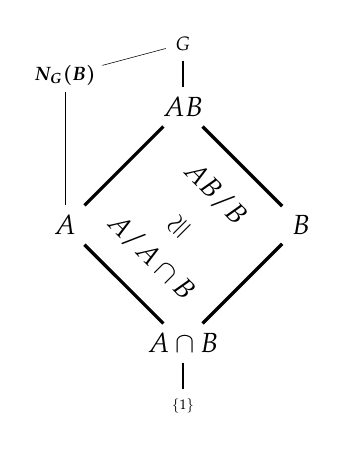
\begin{tikzpicture}
			%	\draw[very thin,densely dashed] (-3,-3) grid (3,3);
			\node (G) at (0,2.3){\scriptsize$G$};
			\node (AB) at (0,1.5){$AB$};
			\node (A) at (-1.5,0){$A$};
			\node (B) at (1.5,0){$B$};
			\node (ab) at (0,-1.5){$A\cap B$};
			\node (e) at (0,-2.3){\tiny$ \{1\} $ };
			\node [scale=.7](NA) at (-1.5,1.9){{\boldmath$ N_G(B) $ }};
			\node at (0,0) {\rotatebox[origin=c]{45}{$ \cong $  }};
			\draw (G) edge[-] (AB)
			(AB) edge[-,very thick] (A)
			(NA) edge[-,very thin](A)
			(NA) edge[-,very thin](G)
			(AB) edge[-,very thick] node [below, scale=1, sloped, yshift=-2mm] {$AB/B$} (B)
			(ab) edge[-,very thick] node [above, scale=1, sloped, yshift= 2mm] {$A/A\cap B$} (A)
			(ab) edge[-,very thick] (B)
			(ab) edge[-] (e);
		\end{tikzpicture}
	\end{center}

	\tbx[Third Isomorphism Theorem\\ (\textbf{quotient of quotient}) ]{if $ H\trianglelefteq G $,
		$ K \trianglelefteq G $ and $ H\ll K $ then $ K/H\trianglelefteq G/H $ and 
		$ (G/H)/(K/H)\cong G/K .$
	}
	\tbx[Fourth Isomorphism Theorem (\textbf{lattice}) ]{ let $N\trianglelefteq G $ (group) then there 
		is a bijection from set of subgroups $ A \ll G$ containing $ N $ to subgroups 
		$ \overline{A}=A/N \ll G/N$ i.e. every subgroup of $ G/N $ is of from $ \overline{A}=A/N $ for some 
		$ A\ll G $ containing $ N $ and this bijection has the following properties : 
		$ \forall A,B \ll G $ with $ N\ll A,B $ we have 
		
			\y  if $ A\ll B $ iff $ \overline{A} \ll \overline{B} $. \\
			\y  if $ A\ll B $ then $ |B:A|=|\overline{B}:\overline{A}| .$ \\
			\y  $ \overline{A\cap B}= \overline{A}\cap \overline{B}. $  \\
			\y  $ A\trianglelefteq G $ iff $ \overline{A} \trianglelefteq \overline{G}. $ 
		
	}
	\subsection{Cayley's Theorem and \\ Class equations}
	\tbx[\textbf{ Cayley's Theorem} ]{every group is isomorphic to a group of permutations (a subgroup
		of a symmetric group)  in particular if $ |G|=n<\infty $  then $ G\cong $ a subgroup of $ S_n $
		\snote{can be derived by left multiplication action of $ G $ on its subgroup $ \{1\} $}.
	}
	\tbx[Consequences of Cayley's theorem]{ 
			\y    if   $ G $ is a finite group of order $ n $, $ p $ is the smallest prime dividing $ n $ and if any subgroup is of 	index $ p $ (if exists) in $ G $ i.e. $ |G:H|=p $ then $ H $ is normal. \\
			\snote{use  left multiplication action of $ G $ on $ \{gH\} $ i.e. $ \pi_H : G\ra S_p $ (permutation representation of the action) whose kernel $ K\ll H $ is such that $ G/K $ isomorphic to a subgroup of $ S_p $ and $|G:K|=|G:H||H:K|  $ so $ |G:K|=pk $ and $ pk|p!\implies k|(p-1)! $ thus $ k=1 $ by minimality of $ p||G| $ so $ K=H $.}\\
			\y Immidieately from preceding point we get \textbf{any subgroup of index $ 2 $ is necessarily a normal subgroup}. \\
			\y  using similar argument as preceding points we get : if $ H $ has finite index in $ G $ i.e. $ |G:H|=n<\infty $ then  
			There exists $ K\ll H $ normal in $ G $ such that $ |G:K|\leq n! .$\\
			\y now if we follow Group action (left multiplication) to find the elements of subgroup of symmetric group that $ G $ is isomorphic to then these elements are called \textbf{left regular representations} of $ G $. \\
			\y  if $ G $ is a finite group then for left regular representation of $ G $ of an element $ x\in G $ of order $ n $ in $ G $ is product of $ m \; n- $cycles only, where $ |G|=nm .$  \\
			\y so for $ \pi:G\ra S_G$ represents the isomorphism stated in Caleys's theorem (by left regular representation)  and  $ x\in G $ $ \phi(x) $ is an odd permutation iff $ |x| $ is even and $ \frac{ |G| }{|\gen{x}|}  $ is odd.\snote{refer symmetric groups}\\
			\y Immediately  from preceding point we get in representation of $ G $ if there exists an odd permutation then $ G $ has a subgroup of index $ 2.$ \\
			\y  if $|G|=2k $ for $ k $ odd then $ G $ has a subgroup of index $ 2 $ i.e. $ \exists H\ll G $ more precisely $ H\trianglelefteq G $ such that $ |G:H|=2 $ ({\footnotesize use preceding 4 points)} 
	}
	
	\tbx[\textbf{The Class Equation} ]{for $ G $ a finite group if $ g_1,g_2,\ck , g_r $ are representatives of distinct conjugacy classes \snote{equivalence class of $ G $ acting on itself by conjugation} of $ G $ not contained in 
		$ Z(G) $ then 
		\begin{center}
			$  |G|=|Z(G)|+\sm{i=1}{r}|G:C_G(g_i)|.$
		\end{center} (an immediate consequence of conjugacy relation).
	}
	\tbx[Consequences of  Class equations :]{
		
			\y  if $ P $ is a group such that $ |P|=p^\alpha $ for $ p $ prime and $ \alpha \geq 1 $  then $ P $ has  
			a non trivial center. i.e. \\
			$ Z(P)\neq 1 $ (and by Lagrange theorem $ |Z(P) |\geq p $)\\
			\y  	now using the preceding point and lattice isomorphism theorem for strong induction on we get : \\ 
			\textbf{for $ p $ prime if $ |G|=p^\alpha $ then there exists a subgroup of order $ p^\beta $ in $ G $ for every
				$ 0\leq \beta \leq \alpha .$}\\
			\y  if $ |G|=p^2 $ for $ p $ prime then $ G $ is abelian as $ P/Z(P) $ is cyclic and more precisely  
			$ Z\cong Z_{p^2} $ or $ Z_p \times Z_p $
		
		
	}
	\subsection{Cauchy's and Sylow's Theorem}
	\tbx[\textbf{Cauchy's Theorem} ]{if $ G $ is finite group such that $ p| |G| $ (prime $ p $) then $ G $ has an element of order $ p .$\\
		{ \footnotesize (use McKay's proof  : form $ p- $tupels from elements of  $ G $ i.e. $ \{(x_1,x_2,\ck,x_p) \}$ such that $ x_1x_2\ck x_p =1 $  and prove cyclic permutation here forms an equivalence relation , whose equivalence classes can have only orders $ 1 $ or $ p $ and there exist more than one element whose equivalence class is singleton. )} 
	}
	\tbx[Consequences of Cauchy's  theorem ]{
		
			\y  \textbf{If $ G $ is finite ablelian group then it has a subgroup of order $ n $ for every +ve $ n $ dividing $ |G| $.} \snote{ use induction : as $ G $ is abelian every subgroup is normal and quotient group is defined. } \\
			\y  any group of order $ P^2 $ is abelian and is of form $ Z_p \times Z_p $ \snote{refer direct products} or $ Z_{p^2} $ 
		
		
	}
	\tbx[\textbf{SYLOW'S Theorem} ]{
		{ Definitions :  for a prime $ p $, $ G $ group\\
			a group of order $ p^\alpha $ is called a $p $-group, subgroups of $ G $ which are $ p $-groups are called 
			$ p $-subgroups.\\
			If $ G $ is group of order $ p^\alpha m $ where $ p \not| m $ (does not divide) then a subgroup of $ G $ or order $ p^\alpha $ is called a Sylow $ p $-subgroup of $ G. $\\
			The set of all Sylow $ p $-subgroups of $ G $ is denoted by $ Syl_p(G) $ and number of  Sylow $ p $-subgroups of $ G $ is denoted by $ n_p(G) $}\\
		\textbf{Theorem} : if $ G $ group has an order $ p^\alpha m $ for $ p\not| m $, prime $ p $ then :
		
			\y  Sylow $ p $-subgroups of $ G $ exists, i.e. $ Syl_p(G)\neq \emptyset $. \\
			\y  if $ P $ is Sylow $ p $-subgroups of $ G $ and $ Q $ is any $ p $-subgroup of $ G $ then $ \exists g \in G $ such that $ Q\ll gPg^{-1} $ i.e. every $ p $-group of $ G $ is subgroup of conjugate of  a Sylow $ p $-subgroups of $ G $ , particularly any two Sylow $ p $-subgroups of $ G $ are conjugates in $ G. $ \\
			\y  $ n_p(G)\equiv 1 \pmod{p} $ i.e. $ n_p(G)=1+kp $ and as $ n_p(G)=|G:N_G(P)| $ we get $ n_p(G) | m .$ }
		
	\tbx[Consequences of of Sylow's Theorem ]{
		if $ P $ is Sylow $ p $-subgroups of $ G $ then $P$ is normal in $ G $ iff $ P $ char $ G .$ iff all subgroups generated by 
		elements of $ p $-power order are $ p $-groups  (i.e. if $ X\subset G $ and $ |x| $is a power of $ p $ for every 
		$ x\in X $ then $ \langle X \rangle $ is $ p $-group) iff $ n_p(G)=1. $}
	
	\subsubsection{ Classification of groups using Sylow's theorem}
	 if $ p,q $ are distinct primes
	\tbx[group $ G $ of order $ pq $ ]{
		
			\y   if $ p<q , Q\in Syl_q(G)$ and $ P\in Syl_p(G) $  then $ Q\trianglelefteq G $ \\ 
			also if $ P\trianglelefteq G $ then $ G\cong Z_{pq}.$(use $ G/C_G(P) \cong $ a subgroup of $ Aut(Z_p) $ and $ p,q\not| p-1 $ to prove $ C_G(P)=G $)	\\
			\y  if $ p<q $ we have $ n_p|q  \implies n_p=1 $ or $ q $  and as $ n_p=1+kp \implies $ if $ p\not| q-1 $ then $ n_p=1 $ so $ P\trianglelefteq G $ and $ G \cong Z_{pq} $  \\
			\y  if $ p|q-1 $ then this is a unique non Abelian group of order $ pq $ }
		
	
	\tbx[group $ G $ of order $ p^2q $]{
			\y  if $ q<p$ then the Sylow $ p $-subgroup is normal in $ G $ (as $ n_p=1 $). \\
			\y  if $ p<q $ then Sylow $ q $-subgroup is normal in $ G $ except for when $ q=p+1 $ i.e. $ p=2 $ i.e. $ |G|=12 $ then $ G $ has either a Sylow - $ 2 $ or a $ 3 $ normal subgroup (use $ n_q|p^2 \implies q|p+1 $). }
	\tbx{ \y if  $ G $ is a finite group of order $ n=p_1p_2\ck p_r $ for distinct primes $ p_i $ such that $ p_i\not| p_j-1\; \forall i,j $  then $ G $ is cyclic. \\
	Converse of preceding point is true i.e. for $ n\geq 2 $ and  if every group of order $ n $ is cyclic then $ n=p_1\ck p_r $  for $ p_i \not| p_j-1. $\\
		Generalising preceding points we get\\
	\y $ Z_n $ is the only group of order $ n $ i.e. number  of groups of order $ n $ is $ 1 $ (cyclic) iff 
	$ gcd(n,\varphi(n))=(n,\varphi(n))=1 $ \\
	\y Every Group of order $ n $ is abelian iff  prime factorization of $ n=p_1p_2\ck p_i q_1^2q_2^2\ck q_j^2 $ for and $ n $ is relatively prime to $ (p_1-1)(p_2-1)\ck (p_i-1) (q_1^2-1)(q_2^2-1)\ck (q_j^2-1).$ 
	\snote{last two points are not a direct consequence but look into Gallian's papers}  }
	 
	\section{Automorphism 
		\\ Theorems}
	\tbx{if $ H \trianglelefteq G$ (group) then $ G $ acts by conjugation on $ H $ as automorphism of $ H $ i.e.
		$ \sigma_g: H\ra gHg^{-1} $ by $ \sigma_g(h)=ghg^{-1} $ is an automorphism. 
	}
	\tbx{now by properties of conjugate action and preceding point we have :\\
		$ \{\sigma_g\}\cong G/C_G(H) $ so $ G/C_G(H) \cong $ subgroup of $ Aut(H) $ if $ H $ is normal in $ G $ 
	}
	\tbx{clearly $ K \trianglelefteq N_G(K) $ so we have \\
		$ N_G(K)/C_G(K) \cong $ a subgroup of $ Aut(K) .$\\
		Particularly $ G/Z(G) \cong $ a subgroup of $ Aut(G) .$
	}
	\tbx{the preceding mentioned subgroup of $ Aut(G) $ formed by conjugation is called inner automorphism of $ G $ denoted by 
		$ Inn(G) .$
	}
	\tbx[\textbf{Characteristic Subgroups }]{Characteristic Subgroups of  $ G $ are subgroup of  $ G $ which remain fixed for every automorphism 
		of $ G $ i.e. $ H  $ char $ G $ iff $ \sigma (H)=H \; \forall \sigma \in Aut(G) $
	}
	\tbx[Properties of Characteristic Subgroups ]{
		
			\y  They are Normal (converse is not true.) \\
			\y  if $ H $ is unique subgroup of order $ n $ in $ G $ (only subgroup of order $ n $) then $ H $ char $ G. $ \\
			\y  if $ K $ char $H$ and $ H\trianglelefteq G $ then $ K\trianglelefteq G .$ \\
			\y  $ H $ char $ K $  and $ K $ char $ G $ then $ H $ char $ G .$  
	}
		\section{Semi Direct product}
	
	\tbx{Motivation :  to Generalise direct product so that not both $ H $ and $ K $ be normal to make a group 
		$ HK $, this helps in building larger groups which have subgroups isomorphic to both $ H $ and $ K $. In this case $ H $ is normal and $ K $ is necessarily not.
		let $ H \trianglelefteq G $ and $ H\cap K=1 $ then there is a unique way of writing elements of $ HK $.
		If we have $ hk \ra (h,k) $ using some map then $ (h_1,k_1)(h_2,k_2)=(h_1k_1)(h_2k_2)=h_1k1h_2 (k_1^{-1}k_1) k_2=h_1(k_1h_2k_1^{-1}) k1k_2= h_3 k_3=(h_3,k_3)$. so if we understand how  $k_1h_2k_1^{-1}  \in H$ without the need of $ G $ then we can define a larger group $ HK $. This needs us to act $ K $ on $ H $ (by conjugation)  
		i.e. a homomorphic map from $ K \ra Aut(H). $ we then define :  if $ k.h= k h k^{-1} $ then $ (h_1k_1)(h_2k_2) 
		= (h_1k_1.h_2)(k_1k_2)$ gets the operation part done for $ HK $
	}
	\tbx{For $  H$,$ K $ be groups, $ \phi :K \ra Aut(H) $ a homomorphism this defines a left action of $ K $ on $ H $ say by $ . $ then let $ G $ be set of ordered pairs $ \{(h,k)|h\in H, k\in K\} $ and define operations on it by 
		$ (h_1,k_1)(h_2,k_2)=(h_1\, k_1.h_2, k_1k_2) $ :
		
		\y  this operation makes $ G $ into a group (\textbf{Semi Direct product}) of order $ |G|=|H||K| $ \\
		\y  for set $ \tilde{H}=\{(h,1)|h\in H\} \ll G$ the map $ h \ra (h,1) $ makes $ H\cong \tilde{H} $  \\
		\y  similarly for set $ \tilde{K}=\{(1,k)|k\in K\} \ll G$ the map $ k \ra (1,k) $ makes $ K\cong \tilde{K} $  \\
		\y  and  $ \tilde{H}\trianglelefteq G$, $ \tilde{H}\cap \tilde{K}= \{1\} $, if $\tilde{h}= (h,1)\in \tilde{H}, \tilde{k}=(1,k)\in \tilde{K} $ then \\
		$ \tilde{k }\tilde{h} \tilde{k}^{-1}=(k.h,1) = (\phi(k)(h),1)$ i.e. action of $ k $ on $ h $ under $ \phi .$
		
		
	}
	\tbx{The preceding group $ G $ can be symbolised (as in case of direct product ) as $ G = H \smdp _\phi S $ or simply $ H \smdp G $ i.e. read as 
		$ G $ semi direct product of $ H $ and $ K $ \snote{ {\small | } on the right of $ \smdp $denotes that $ H \trianglelefteq G $}
	}
	\tbx{$ H \smdp G = H \times G $
		
		\y  iff $ \phi : K \ra Aut(H) $ is trivial i.e. $ \phi(k)=1 \, \forall k \in K.$  \\
		\y  iff $ K \trianglelefteq H\smdp K .$ \\
		\y  iff $ \psi : H\smdp K \ra H\times K  $ by $ (h,k) \ra (h,k) $ (i.e. identity map) is homomorphism (in fact isomorphism.) 
		
		
	}
	\tbx[Recognition Theorem of Semi Direct product]{ if $ H,K \ll G $ are such that $ H\trianglelefteq G $ and $ H \cap K =1 $ then by $ \phi  $ action of conjugation of  $ K $ on $ H $ in $ G $ we have 
		\begin{center}
			$ HK\cong H \smdp K .$
		\end{center}
	}
	\tbx{For $ H\ll G $, $ K \ll G $ is called \textbf{Compliment } of $ H $ in $ G $ if $ H\cap K =1 $ and $ G=HK $
	}
	\subsection{Examples}
	\tbx{
		Group $ G $ of order $ pq $  for $ p,q $ distinct primes: by Sylows theorems we have at least one of the Sylow subgroup is normal, say $ p<q $ then $ Q= Syl_q(G) \trianglelefteq G$ and $ Aut(Q) $ is cyclic group of order $ q-1 .$\\
		\textbf{case 1} : if $ p\not|q-1 $ then $ \phi :  Syl_p(G)=P\ra Aut(Q)$ is trivial so $ G= PQ=P\smdp Q = P \times Q $ this makes $ G $ cyclic as stated earlier.\\
		\textbf{case 2} : if $ p|q-1 $ as $ Aut(Q) $ is cyclic it contains a unique subgroup (cyclic) of order $ p $ say 
		$ \gen{\gamma }$ so any homomorphism $ \phi_i : P \ra Aut(Q)  $ is given by $ \phi_i(x)=\gamma^i $ for $ P=\gen{x}, 0\geq i \geq p-1 $. Now $ \phi_0 $ is trivial so goes to case 1. if $ i\neq 0 $ then each $ \phi_i $ gives raise to non-abelian group $ Q \smdp_{\phi_i} P $, but all these groups are isomorphic as the  any non trivial homomorphisms of $ |P|=p = |\gen{\gamma}|$ maps generators map to generators. Thus all these semi direct product groups are same.\\
		\textbf{Finally we  have there are only two unique groups of order $ pq $ one cyclic and other the non trivial semi direct product of its sylow subgroups.}}
	
	\tbx[\small Class equation of non abelian $pq $ order group]{ now for the unique non-abelian group of order $ pq $ for $ p|q-1 $ we have $ n_p=q$ and as each element of sylow $ p $ subgroup is transferred to one (non identity) element of other sylow $ p $ group by conjugation and as sylow $ p $ group $ \cong Z_p$ (abelian) we have each element other than $ e $ of sylow $ p $ subgroup has  $ q $ elements in conjugacy class i.e. $ q $ is repeated $ p-1 $ times, now as  $ Q= $ sylow $ q $ subgroup is normal and $ \cong Z_q $ we have $ |Inn(Q)|=|G/C_g(Q)|=|G/Q|=p $ so $ p $ elements in one class and number of distinct classes equal to partition of $ q-1 $ non identity elements of $ Q $ into each $ p $ element part sets i.e. $ q-1/p $  distinct classes. From this we get \\
		$ |G|=pq$
		\begin{center}
			$=1+\underbrace{p+p+\ck +p}_{\frac{ q-1 }{p}\w{ times}}+\underbrace{q+q+\ck+q}_{p-1 \w{ times}} .$
	\end{center}  }
	
	
	\tbx{ Group $ G $ of order $ p^3 $ for $ p $ an odd prime : 
		assume $ G $ is not cyclic then \\
		if $ G $ is not abelian then $ |Z(G)|=p $ only by class equation and fact that if $ P/Z(P) $ is cyclic then $ P $ is abelian.\\
		defining a $ p $th power map $ x\ra x^p $ gives a homomorphism from $ P\ra Z(P) $ and with kernel of size only $ p^3 $ or if this kernel is $ p^2 $ then there is an element of order $ p^2 $\\
		case 1 : $ G $ has a element $ x $ of order $ p^2 $ \\
		let $ H=\gen{x} $ then $ H $ is prime index in $ G $ so $ H \trianglelefteq G $, if $ E$ is kernel $  p$th power map then $ E \cong Z_p \times Z_p $ as every $ x\in E \; x^p=1$ clearly $ E \cap H =<x^p> .$\\
		now if $ y\in E-H $ then for $ K=\gen{y} $ we have $ H \cap K=\{1\} $ and $ G =H \smdp K $ thus 
		$ G \cong Z_{p^2} \smdp Z_p $ for some $ \phi : K \ra Aut(H) $ if $ \phi $ is trivial then $ G \cong Z_{p^2}\times Z_p $ which is abelian so for non trivial $ \phi $ there exists a unique non abelian $ H \smdp K $ (the non trivial ones are isomorphic as $ K $ is of order $ p $)\\
		case 2 : every non identity element is of order $ p .$
		so  for any subgroup of $ H $ if is of order $ p^2 $ then $ H=Z_p\times Z_p $ and clearly $ H \trianglelefteq G $ (as prime index) , if $ K=\gen{y} $ for some $ y\in G-H $ then $ |K|=p $ and $ H\cap K=\{1\} $ thus $ G=H\smdp K $ i.e. $ G \cong (Z_p\times Z_p)\smdp Z_p $ for some $ \phi : K \ra Aut(H) $ by similar reasoning if $ \phi  $ is trivial then $ G \cong Z_p\times Z_p\times Z_p $ which is abelian , only other possibility  is a non abelian $ G $\\
		\textbf{	Thus the only groups of order $ p^3 $ upto isomorphism are : \\
			abelian : cyclic, $ Z_{p^2}\times Z_p $,  $ Z_p\times Z_p\times Z_p $ \\
			and non abelian  : $Z_{p^2}\smdp Z_p $, $  (Z_p\times Z_p)\smdp Z_p  $ for some non trivial $ \phi  $ homomorphism from $ Z_p $ to its complement.}
	}
	\tbx[Class equation for group of order $ p^3 $]{ 
		clearly $ |Z(G)|=p $ now if $ g\not\in Z(G) $ then $ g\in C_G(g) $ and $ Z(G)\ll C_G(g) $ but $ C_G(g)\neq G $ so only possibility remaining is $ |C_G(g)|=p^2 $ so $ |G:C_G(g)|=p $ now calculating we get\\
		$ |G|=p^3=\underbrace{1+1+\ck+1}_{p \w{ times}} +\underbrace{p+p+\ck+p}_{p^2-1\w{ times}}.$}
	\subsection{$ p $-groups and Fundamental theorem of finite abelian groups}
	
	\tbx{a group of order $ p^\alpha $ for $ p $ prime and $ \alpha \geq 1 $ is called a $ p $-Group.
	}
	\tbx{for a $ p $-Group of order $ p^a $ 
		
		\y  $ Z(P) \neq \{1 \}.$ i.e. center of $ P $ is not trivial \\
		\y  for non trivial $ H \trianglelefteq P $ then $ H \cap Z(P) \neq 1 .$ \\ 
		\snote{ In particular every normal subgroup of order $ p $ of $ P $ is contained in $ Z(P) .$}\\
		\y  for $ H \trianglelefteq P $ and if $ p^b | |H| $ then $ H $ contains a group of order $ p^b $ which is normal in $ P $ (In particular $ P $ has a normal subgroup of order $ p^b $ for every $b \in \{0,1,\ck , a\} $) \\
		\y  if proper $ H \ll  P $ then proper $ H \ll N_P(H) $ i.e. every proper subgroup of $ P $ is a proper subgroup of its normaliser in $ P .$ \\
		\y  Every maximal subgroup of $ P $ is of index $ p $  and is normal. 
		
		
	}
	\tbx{{\large \textbf{Every finite abelian group is a direct product of its Sylow subgroups} }\\
		\snote{if finite abelian $ G $ is such that $ |G|= p_1^{k_1}p_2^{k_2}p_3^{k_3}\ck p_r^{k_r} $ for distinct primes $ p_i $ then $ P_1=Syl_{p_1}(G), P_2=Syl_{p_2}(G) \trianglelefteq G$ and $ P_1 \cap P_2 =\{1\} $ as $ p_1 \not| p_2 $ thus $ P_1P_1\cong P_1 \times P_2 $ now $ P_3=Syl_{p_3}(G) \trianglelefteq G$ and $ P_1P_2 \cap P_3 =\{1\}$ as $ p3\not| p2,p3 \not|p1 $ thus $ P_1P_2P_3\cong P_1 P_2 \times P_3 \cong P_1\times P_2 \times P_3 $ continuing this process till $ P_r $ we get by an order argument $ G=P_1P_2P_3\ck P_r \cong P_1 \times P_2 \times P_3 \times \ck \times P_r .$}
	}
	\tbx{if  $G $ is an abelian $ p $ group then for $ a\in G $ with maximal order we have 
		\begin{center}
			$ G= \gen{a}\times K .$
		\end{center}where $ K $ is the complement of $ \gen{a} $ in $ G $ \\
		\snote{use induction : choose $ b\notin \gen{a} $ of minimal order and prove $ \gen{a}\cap \gen{b}=\{1\},|\gen{b}|=p $, for $ G/\gen{b} $ if  $\,\bar{\quad} \,$ represents the corresponding elements in $ G/\gen{b} $ prove $ |\overline{a}| =|a|$  so $ \overline{a} $ is maximal order thus $ \overline{G}=\overline{a}\times \overline{K} $ pull back $ \overline{K} $ to $ K $ in $ G $ , prove $ \gen{a}\cap K =\{1\} $ and claim $ G=\gen{a}\times K $ by order argument .}
	}
	\tbx{an Immediate consequence of preceding point :\\
		\textbf{ Every $ p $-Group is the direct product of its cyclic subgroups.}\\
		From Last three points we get a Fundamental theorem of finite abelian Groups :
	}
	\tbx[\textbf{ Fundamental theorem of finite abelian Groups} ]{elementary divisors decomposition form :  
		if $ G $ is an abelian group of order $ n=p_1^{\alpha_1}p_2^{\alpha_2}\ck p_k^{\alpha_k} $ then :
		
		\y  $ G \cong A_1 \times A_2 \times \ck \times A_k $ where $ |A_i|=p_i^{\alpha_i} .$ \\
		\y  each $ A_i \cong Z_{p_i^{\beta_{i1}}} \times Z_{p_i^{\beta_{i2}}}\times \ck \times Z_{p_i^{\beta_{it}}}$  with  
		$ \beta_{i1}\geq \beta_{i2} \geq \ck \geq \beta_{it} $ and $ \beta_{i1}+\beta_{i2}+\ck +\beta_{it} = \alpha_i $\\
		\snote{$ p_i^{\beta_{ij}} $ are called elementary divisors of $ G $}\\
		\y  This decomposition is unique (till isomorphism.) 
		
	}
	
	\tbx[\textbf{Fundamental theorem of finite abelian Groups} ]{invariant factors decomposition form :
		Every finite abelian group $ G $ is of unique  decomposition form (till isomorphism) given by 
		\begin{center}
			$ G \cong Z_{n_1} \times Z_{n_2} \times \ck \times Z_{n_s}.$
		\end{center}
		With $ n_j \geq 2\, \forall i$ and $ n_{i+1}|n_i  \w{ for } 1\leq i \leq s-1$
	}
	\tbx{for $ m,n \in \Z^+ $ 
		
		\y  $ Z_m \times Z_n \cong Z_{mn} $ iff $ (m,n)=1 $ \\
		\y  if $ n=p_1^{\alpha_1}p_2^{\alpha_2}\ck p_k^{\alpha_k} $ then \\ 
		$ Z_n=Z_{p_1^{\alpha_1}}\times Z_{p_2^{\alpha_2}}\times\ck\times Z_{p_k^{\alpha_k} }.$
		\\ From this theorem we can Change the forms of a Fundamental theorem of finite abelian Groups.
		
	}

	\section{Presentations}
	
	\tbx{A presentation of a group is a compact way of stating the properties  of  group from  which the group it self can be derived 
	}
	\tbx{\textbf{Generators} a group $ G $ is said to be generated by a subset $ A=\{a_1,a_2,\ck , a_n\} $ if every element of $ G $ is a combination of these elements (by group operation) and is denoted by 
		$ G=\langle A \rangle =\langle a_1,a_2,\ck ,a_n\rangle  $
	}
	\tbx{Every finite group has a finite generating set (consider the group itself)
	}
	\tbx{The properties that these generators holds holds even for the group and the converse is also true the properties possessed by the group is the properties fo these generators too. Thus if we know all the generators and all their properties it is enough to in a sense to know the whole group itself all other properties of the group can be derived from these so if $ a_1,a_2,\ck ,a_n $ are generators of $ G $ with properties $ P_1, P_2, \ck P_m $ only then $ G $ can be stated as $ \gen{a_1,a_2,\ck ,a_n| P_1,P_2,\ck ,P_m} $
		and this is called \textbf{Presentation} of $ G $ in a sense the presentation is `complete' or is made `complete' by adding properties i.e. whole of $ G $ the group and the corresponding group operation can be derived from the Presentation of $ G. $
	}
	\tbx{To denote presentations (`complete') we use
		$ G \pst \gen{a_1,a_2,\ck ,a_n| P_1,P_2,\ck ,P_m}$
	}
	\tbx{examples 
		\begin{center}
			$ Z_n \pst \gen{x|x^n=1} $\\
			$ D_{2n} \pst \gen{r,s|r^n=s^2=1, \, rs=sr^{-1}} $\\
			for $ d=(m,n) $\\
			$ Z_m\times Z_n \pst \gen{x,y|x^n=y^m=1,xy=yx, x^{n/d}=y^{n/d}} $
	\end{center}}
	
	\section{Major Group \\ examples and their Properties}
	\subsection{Cyclic Group} 
	
	\tbx{	Cyclic groups can be viewed as quotient groups of	$ \Z $ formed by $\{kn|k\in \Z\}= n\Z \ll Z$ for $ n\in \Z $ i.e. 
		$ \Z/n\Z = \{ \overline{0},\overline{1},\ck , \overline{n-1}\}$ where $ \overline{s}=\{q\in \Z|q\pmod n =s\} $ and 
		$  (\Z/nZ,\oplus)\cong Z_n$ where $ \oplus $ is modulo addition w.r.t $ n $ i.e.
		$ a\oplus b = (a+b )\pmod{n} $. All properties of this group is same as any cyclic group of same finite order. \\
		Infinite cyclic group $ \Z $ whose generators are $ \{1,-1\} $ only.}
		\tbx{ Homomorphism $ \psi $ \textbf{from }a cyclic group is completely determined by $ \psi(a) $ for a generator $ a $ of the cyclic group.  }
		\tbx{\y Number of Homomorphism from $ \Z/m\Z\ra \Z/n\Z $ is equal to $ (m,n)=gcd(m,n) $ 
		\snote{use: if $ \psi  :\Z/m\Z\ra \Z/n\Z$ is a homomorphism such that  $ a \ra \psi(a) $ for some generator $ a $ of $ \Z/m\Z $ then $ |\psi(a)|\mid m ,\; |\psi(a)|\mid n $   thus $ |\psi(a)| \mid (m,n)$ so $ a $ maps to a generator of subgroup of $ \Z/n\Z $ whose order divides $ (m,n) $ say $ d $, the number of such generators $ =\varphi(d) $ so number of homomorphisms $ =\sm{d|(m,n)}{}\varphi((m,n))=(m,n) $ }  }
	\subsection{$ (\Z/n\Z)^* $}
	
	\tbx{Define a group $ (\Z/n\Z)^* $ subset of $ Z/n\Z $   (not subgroup) with operation $ \otimes $ i.e. $ a\otimes b= (ab)\pmod{n} $ and $ (\Z/n\Z)^* =\{i<n|(i,n)=1\} $ i.e. $ i<n $ such that $ i $ is relative prime to $ n $
		and $ Aut(\Z/n\Z)\cong  (\Z/n\Z)^* $
	}
	\tbx{$ | (\Z/n\Z)^*|=\varphi(n) $
	}
	\tbx{$  (\Z/2^n\Z)^* $ is not cyclic for $ n\geq 3 $ \\ 
		\snote{as $ (2^n-1,2^n) =1 $,$ (2^{n-1}-1,2^n)=1$ but 
			$ (2^n-1)^2\equiv 1 \pmod{2^n} $ and  	$ (2^{n-1}-1)^2\equiv 1 \pmod{2^n} $ \\
			so  $ |<2^{n-1}-1>|=|<2^{n}-1>|=2 $}
	}
	\tbx{for every odd prime $ p $ and $ n\geq 1$
		\begin{center}
			$ (\Z/p^n\Z)^* $ is a cyclic group of order $ p^{n-1}(p-1) $ 
		\end{center} \snote{ use ring theory.}}
	
	\subsection{Dihedral Groups}
	
	\tbx[Motivation]{\footnotesize 
		given a $n$-regular (equal sides) polygon the ways in which it can be moved
		or transformed via rigid motions (no tear or distortions like stretch) to obtain the same 
		figure (symmetric to original position). We call these transformations symmetries, to 
		visualize them we can mark each vertex (corner) with fixed number starting from $1$ to $n$ 
		in a clockwise fashion and see how symmetries change the positions of these numbers.
		
			\y  for example if $r$ a symmetry that rotates the polygon by $2\pi/n$ degrees clockwise,  
			changes the position of numbers like $ 1$ goes to position where $2$ was i.e. $1\ra 2$,
			similarly $i\ra i+1$ for $1\leq i<n$ and $n\ra 1$ \\
			\y  This motion can be replicated counter-clockwise also and the flip or mirroring of  
			positions via a line of symmetry also constitute such motions.\\
			\y  all these motions can be condensed in to just two motions and their combinations: \\
			\y  $r$ a rotation clockwise by $2\pi/n$ \\
			\y  $s$ a flip (change of position from left to right vis-a-vis like a mirror) through 
			the line of symmetry between vertex $1$ and centre of the polygon \\
	\y \textbf{Group concept} These motions from a group if we regard identity as the one fixed starting position and 
		composition of motions as binary operations.\\
		 I.e. for a $n$-regular polygon the group formed by symmetries (rigid motions)
		constitute a group under composition}
	\tbx{This group is made up of $r$ and $s$ motions and their combinations, Properties and 
		derivation:
		
			\y  $r^n=e$ (Identity), $s^2=e.$ \\
			\y  $s\neq r^j$. \\
			\y  $sr^j\neq sr^i\; (i\neq j).$ \\
			\y  $(r^i)^{-1}=r^{n-i}$, $s^{-1}=s.$ \\
			\y  $rs=sr^{-1}$ so by induction 
			\begin{center}
				$r^is=sr^{-i}.$
			\end{center}
			\y  from preceding points we get: 
			\begin{center}
				Dihedral group of $n$-regular polygon = \\
				$D_{2n}=\{e,r,r^2,\ck,r^n-1,s,sr,sr^2,\ck,sr^{n-1}\}.$
			\end{center} here $2n$ signifies the order of the group 	}
		
	\tbx[Properties of $D_{2n}$ ]{
			\y  $\{r^i|0\leq i<n\}$, $\{e,s\}$ forms Cyclic subgroups (there are many other cyclic,  
			non cyclic-subgroup).\\
			\y  if $n$ is odd only $e$ commutes with every element. \\
			\y  if $n$ is even only $e,r^{n/2}$ commutes with every element. \\
			\y  if $G$ is any finite group generated by two distinct elements $x,y$ for order of $ y =\;2$ then $G\cong D_{2n}$ where $n=|xy|$ \\
			\y \textbf{also if $ |G|=2p $ for a prime $ p $ and is non abelian then $ G\cong D_{2p} $  }}

\tbx[Class equation]{ for $ D_{2n} $ we have \\
\y if $ n $ is even then : $ \{e,r^n/2\}=Z(D_{2n}) $, for every $ r^i,\; $ $ r^j r^i r^{n-j}=r^i $ , $ sr^is=r^{-i}=r^{n-1} $ and $ sr^jr^i r^{-j}s=r^{-i} $ so for given $ n-2 $ $ r^i $ variables have a conjugacy class of order $ 2 $ so a total of $ n-2/2 $ classes , for $ s,\; $ $ r^jsr^{-j}=sr^{n-2j} $ now as $ n $ is even $ n-2j $ is even so conjugacy class of $ s  =\{sr^{2i}\} $ and for $ sr,\;$ $ r^jsrr^{-j} =sr^{n-2j+1}$ so conjugacy class of $ sr $ $ =\{sr^{2i+1}\} $ from this we get class equation
\begin{center}
	$ |D_{2n}|=1+1 +\underbrace{2+2+\ck+2}_{\frac{ n-2 }{2} \w{ times}}+\frac{ n }{2} +\frac{ n }{2} $
	\end{center}   
\y if $ n $ is odd most remain same but  as $ \{e\}=Z(D_{2n}) $ , $ n-1/2 $ conjugacy classes of $2$ elements and only one remaining class with $ n $  elements (class of $ s $) so we get class equation
\begin{center}
	$ |D_{2n}|=1+\underbrace{2+2+\ck+2}_{\frac{ n-1 }{2} \w{ times}}+{ n }$
\end{center}   
}
\tbx[Semi direct product construction of $ D_{2n}=H\smdp K $  ]{ \y clearly $ \gen{r} $ is of index $ 2 $ so normal in $ D_{2n} $ so $ H=\gen{r}= Z_n$ and $ K=Z_2 $ only possibility left\\
\y  we know $ rs=sr^{-1} $ i.e. $ srs=r^{-1} $ or $ sr^is=r^{-i} $ so define automorphism $ \phi : K\ra Aut(H)  $ by $x.y=y^{-1}  $ \\
\y thus we have $ D_{2n}\cong Z_n\smdp Z_2 $ }
	\subsection{Symmetric Groups}
	
	\tbx{Motivation : every element in a finite or countably finite set can be numbered so
		representing each element with a number makes sense the bijections (maps) of these sets 
		form a group these can be represented as permutations or rearrangements of numbers.
	}
	\tbx{Group concept : for a given set $A$ the bijections (maps) on this set given by $S_A$ 
		forms a group under function composition : identity map acts as identity, clearly 
		composition of two bijections is another bijection, every bijection has an inverse which is
		a bijection
	}
	\tbx{for set $\Omega=\{1,2,\ck,n\}$ the bijections on this or Symmetric group of this group is
		$S_n$ and clearly $|S_n|=n!$}
	\subsubsection{Cycles} 
	
	\tbx{each bijection $\sigma$ of $\Omega$ can be represented as the following :\\
		$\sigma=(\!a_1,a_2,\ck,a_{(\!m_1\!)}\!)(\!a_{(\!m_1\!)+1},a_{(\!m_1\!)+2},\ck\\
		,a_{(\!m_2\!)}\!)\ck(\!a_{(\!m_k\!)+1},a_{(\!m_k\!)+2},\ck,a_{m_{(\!k+1\!)}}\!)$
		which can be read as (if $\ra$ indicates maps to) 
	\begin{flushleft}
		\begin{tikzpicture}[scale=.65]
	%		\draw [thin,densely dashed](-2,2)grid(2,-2);
	%			\draw[dashed] (0,0) circle [radius=2];
	\node (a1) at (0,2) {$a_1$};
	\node (a2)  at (1.732,1) {$a_2$};
	\node (am)  at (-1.732,1) {$a_{(m_1)}$};
	\draw[thick,->](a1)  to[bend left=21] (a2);
	\draw [thick,->] (a2) to[bend left=11]  (2,0);
	\draw[thick,loosely dotted] (2,0) arc [radius = 2, start angle = 0, end angle =-180];
	\draw[thick,->] (-2,0) to[bend left=9] (am);
	\draw[thick,->](am)  to[bend left=21] (a1);
	
	\node at (2.3,0) {$,$};
	
	\coordinate (xp) at (5,0);
	\node (am1) at  ($(a1)+(xp)-(.1,.1)$)  {$a_{(m_1)+1}$};
	\node (am2)  at ($(a2)+(xp)-(-.2,.2)$) {$a_{(m_1)+2}$};
	\node (amm)  at ($(am)+(xp)-(.2,.2)$) {$a_{(m_2)}$};
	\draw[thick,->](am1)  to[bend left=21] (am2);
	\draw [thick,->] (am2) to[bend left=11]  ($(2,0)+(xp)-(-.2,.2)$);
	\draw[thick,loosely dotted] ($(2,0)+(xp)-(-.2,.2)$) arc [radius = 2.2, start angle = 0, end angle =-180];
	\draw[thick,->] ($(-2,0)+(xp)-(.2,.2)$)  to[bend left=9] (amm);
	\draw[thick,->](amm)  to[bend left=21] (am1);
	
	\node at (8,0) {\footnotesize$,\ck,$};
	
	\coordinate (xp1) at ($(.7,-5)$);
	\coordinate (xpp) at ($(.7,-5)$);
	\node (b1) at  ($(a1)+(xpp)-(.1,.1)$)  {$a_{(m_k)+1}$};
	\node (b2)  at ($(a2)+(xpp)-(-.2,.2)$) {$a_{(m_k)+2}$};
	\node (bm)  at ($(am)+(xpp)-(.2,.2)$) {$a_{(m_{k+1})}$};
	\draw[thick,->](b1)  to[bend left=21] (b2);
	\draw [thick,->] (b2) to[bend left=11]  ($(2,0)+(xp1)-(-.2,.2)$);
	\draw[thick,loosely dotted] ($(2,0)+(xp1)-(-.2,.2)$) arc [radius = 2.2, start angle = 0, end angle =-180];
	\draw[thick,->] ($(-2,0)+(xp1)-(.2,.2)$)  to[bend left=9] (bm);
	\draw[thick,->](bm)  to[bend left=21] (b1);
	
\end{tikzpicture} 
\end{flushleft}
	where $a_i$'s are distinct elements of $\Omega$}
	
	\subsubsection{ Properties of Cycles and cycle decompositions:}
	
	\tbx{cycles can be composed similar to corresponding bijections and the results in both case are 
		same ({\footnotesize note : composition of cycles are simplified right to left )}.
	}
	\tbx{disjoint cycles commute.
	}
	\tbx{order of a $m$-cycle (of length $m$ or consisting of $m$ elements) is $m$
	}
	\tbx{order of a bijection with disjoint cycles representation is the l.c.m of lengths of the 
		cycles in its representation.
	}
	\tbx{\textbf{Cycle Type} : for $ \sigma \in S_n $ is a product of $ n_1,n_2,\ck , n_r $ cycles (including 1-cycle) such that $ n_1\geq n_2 \geq \ck \geq n_r $ then integers $ n_1,n_2,\ck , n_r $ are called the cycle type of $ \sigma $
	}
	\tbx{\textbf{Partition of $ n\in \Na $} is a non decreasing sequence of +ve integers summing up to $ n. $
	}
	\tbx{a bijection has order $p$ prime iff it is represented as product of commuting $p$-cycles.
	}
	\tbx{if $ \sigma,\tau \in S_n$ and $ \sigma $ has a cycle decomposition $ (a_1,a_1,\ck, a_{k_1})(b_1,b_2,\ck ,b_{k_1}),\ck $ then
		\begin{center}
			$ \tau \sigma \tau^{-1} $ has cycle decomposition\\
			$(\tau(a_1),\tau(a_1),\ck, \tau(a_{k_1}))$\\
			$(\tau(b_1),\tau(b_2),\ck ,\tau(b_{k_1})),\ck   .$
		\end{center} (use if $ \sigma(i)=j \implies  \tau \sigma \tau^{-1} (\tau(i))=\tau(j)$ thus if $ i,j $ appear in $\sigma\implies\; \tau(i),\tau(j)$ appear in $\tau$'s cycle decomposition).
	}
	\tbx{From preceding point we get 2 elements of $ S_n $ are conjugates iff they have same cycle type.
	}
	\tbx{and from preceding two point we get the number of conjugacy classes of $ S_n $ are equal to the partitions of $ n .$ (note here we include even 1-cycles)
	}
	\tbx{if $ \sigma \in S_n $ and $ \sigma $ is decomposed into (distinct) $ m_1,m_2,\ck, m_r $ cycles (including 1-cycle) with multiplicity (number of cycles for a fixed length) of $ k_1,k_2,\ck , k_r $ 
		(so $ n= \sum_{i=1}^{r}k_im_i $ , $ \sigma $ consists of $ k_i $ $ m_i $-cycles which are disjoint) then the number of permutations of cycle type $ \sigma $ or the number of elements in the conjugacy class of $ \sigma $ is equal to 
		\begin{center}
			$ \frac{ n! }{(k_1!m_{1}^{k_1})(k_2!m_{2}^{k_2})\ck (k_r!m_{r}^{k_r})}=\frac{ n! }{\prod_{i=1}^{r}k_i!m_i^{k_i}} .$
		\end{center}
	}
	\tbx{from preceding point we have, if $ K $ is a transposition conjugacy class of $ S_n $ and $  K' $ is any other conjugacy class on an element of order $ 2 $ that is not a transposition of $ S_n $ then except for $ n=6 \; (S_6)$ $ |K|\neq |K'| $ (for $ S_6 $ $ |K|=15 $ and for class $ 3 $ disjoint transposition $ |K'|=15 $ only exception).
	}
		\tbx{from preceding two points we have :
		\begin{center}
			$ Aut(S_n)=Inn(S_n) .$
		\end{center} with only exception of $ S_6 $ \\ where $ |Aut(S_6):Inn(S_6)|=2 $ \\
		{ \footnotesize (use if $ \sigma \in Aut(S_n) $ then for a conjugacy class $ K $ $ \sigma(K) $ is also a conjugacy class, so transpositions are mapped to transpositions except in $ S_6 $, $ \sigma((1,2))=(a,b_1), \sigma((1,3))=(a,b_2),\ck, \sigma ((1,n))=(a,b_n)$ only , and these permutations generate $ S_n $ so $ Aut(S_n) $ has at most $ n! $ order= order of $ Inn(S_n) $).}}
		
	\tbx[Class equation]{ from all preceding points we get if $ n\geq 3 $ \snote{ as $ S_2\cong Z_2 $}
	\begin{center}
		$ |S_n|= 1+\sum\limits_{p_i}\left(\frac{ n! }{\prod_{i=1}^{r}k_{ij}!m_{ij}^{k_{ij}}}\right).$ 
		\end{center}  
	where $ p_i's $ are distinct partitions of $ n $ such that $ p_ i$ has disjoint $ k_{ij} $ cycles of cycle length $ m_{ij} $ i.e $ n=\sum_j k_{ij}m_{ij}$ }
	\tbx[Greatest order element in $ S_n $ ]{
	\y order of element is equal to the lcm of lengths of disjoint cycles \\
	 \y so for given $ n $ we need to partition $ n $ into primes and multiply the primes in partition to get the order and find a partition of $ n=p_1+p_2+\ck +p_k =\sm{i=1}{k}p_i$ for $ p_i $ primes such that 
	 $ p_1p_2\ck p_k=\prod\limits_{i=1}^{k}p_i$ is maximum.\\
	 \y by number theory we have the products of parts in partition is maximum if each part tends to $ e $ and number of parts tends to $ n/e $ so if $ g(n) $ represents the greatest order element in $ S_n $  then we have 
	 \begin{center}\large
	 	$ g(n)<e^{\frac{ n }{e}  } .$
	 	\end{center}  }

	\subsubsection{Transpositions and Alternating Group} 
	
	\tbx{a two cycle is called a transposition.
	}
	\tbx{Every element of $ S_n $ can be made into product of transpositions (not necessarily distinct )\\
		for eg : a cycle 
		\begin{center}
			$ (a_1,a_2,\ck,a_m) =(a_1,a_m)(a_2,a_m)\ck (a_{m-1},a_m).$
		\end{center}
	}
	\tbx{let $ x_1,x_2,\ck ,x_n $ be $ n $ independent  variables then we define :
		\begin{center}
			$ \triangle =\prod\limits_{1\leq i \leq j \leq n} (x_i - x_j) ,$\\
			and for $ \sigma \in S_n $\\
			$ \sigma (\triangle )=\prod\limits_{1\leq  i \leq j \leq n} (x_{\sigma (i)} - x_{\sigma (j)} ) .$
			Then we get (by rearranging) 
			$ \sigma (\triangle)= \pm \triangle.$ 
		\end{center}
	}
	\tbx{Again we define a function : sign of $ \sigma \in S_n $ i.e. $ \epsilon : S_n \ra \{-1,1\}  $ as \\ 
		$ \epsilon(\sigma) =
		\begin{cases}
			+1 ,\qquad \w{if } \sigma(\triangle) = \triangle \\
			-1 ,\qquad \w{if } \sigma(\triangle) = -\triangle 
		\end{cases} $ }
	
	\tbx{we call (define) $ \sigma \in S_n $ is even permutation if $ \epsilon(\sigma)=1 $ or an odd permutation if 
		$ \epsilon(\sigma)=1 $ 
	}
	\tbx{map $ \epsilon : \,S_n \ra \{\pm 1\} $ is a homomorphism (if $ \{\pm 1\}  $ is assumed as multiplicative group)
	}
	\tbx[Alternating Group]{so an Alternating group of degree $ n $ denoted by $ A_n $ is the kernel of this homomorphism
		(i.e. set of all even permutations in $ S_n $)
	}
	\tbx[Classifying methods :]{
		
			\y  a transposition is an odd permutation \\
			\y  every $ n $-cycle can be decomposed as product of $ n-1 $ transpositions. \\
			\y  so a $ m $- cycle is odd permutation iff $ m $ is even and\\ 
			vis-a-v  a $ m $- cycle is even permutation iff $ m $ is odd\\
			\y  from preceding points we get :\\ 
			\textbf{a permutation $\sigma$ is odd iff the number of cycles of even length in its cycle decomposition is odd} and vis-a-v for a permutation to be even.
				}
\tbx{\textbf{every $ A_n $ for $ n\geq 5 $ is a simple group.}}
	\subsection{Quaternion Group}
\tbx{ let $ Q_8=\{1,-1,i,-i,j,-j,k,-k\} $ define group operations as
	
	\begin{center}

	$ \forall a\in q_8,1.a=a.1,-1.-1=1,-1.a=-a $ \\
	$ i.i=j.j=k.k=-1 $ \\
	$ \begin{matrix}
		i.j=k,& j.i=-k\\
		j.k=i,& k.j=-i\\
		k.i=j,& i.k=-j
	\end{matrix} $  
		
\end{center}
}
\tbx{ 
\y clearly $ Q_8 $ is non-ablelian\\
\y $ Z(Q_8)=\{1,-1\} $ \\
 \y $\gen{i},\gen{j},\gen{k}$ are 3 normal subgroups of order $ 4 $ in $ Q_8 $ }
 \tbx[Generalised Quaternion Group ]{ (refer semi-direct product and presentations)\\
 \y let $ H=\gen{h}\cong Z_{2^n} $, $ K=\gen{x}\cong Z_4 $  the form $ H\smdp K $ by $ G= K\ra Aut(H) $ by inversion i.e. $ x.h=h^{-1} $ i.e. $ xhx^{-1}=h^{-1} $ \\
\y so $ x^2\in  Z(G) $  and if $ z=h^{2^{n-1}} $ then $ \gen{z} $ is a unique subgroup of order $ 2 $ in $ H $ and $ x $ inverts this i.e. $ xzz^{-1}=z^{-1}=z $ thus $ x $ centralizes $ z $ so we have $ z\in Z(G) $ as $ z $ commutes with both $ x,h $. now $ x^2z\in Z(G) $ so we have $ \gen{x^2Z}\trianglelefteq G $.\\
 \y Now form the quotient group $ \overline{G}=G/\gen{x^2z}$ let bar indicate this transition so we have\\
 $ \overline{x} $ inverts $ \overline{h} $ (property inherited from $ G $) and $ |\overline{G}|=|G|/|\gen{x^2z}|=|G|/2=2^{n+1} $ \\
 if $ n=2 $ we have $ {x}^2{h}^{2}\in \gen{x^2z}\implies {x}^2{x}^2{h}^{2}\in x^2\gen{x^2z}$ i.e. $ h^2 \in x^2\gen{x^2z}$ so we have $ \overline{x}^2=\overline{h}^2 $ which implies $ \overline{G}\cong Q_8 $ \\
\y Thus the General Quaternion Group is given by the Quotient group $\overline{G}$ and is presented as 
\\ $ Q_{2^{n+1}} \pst \gen{ h,x |h^{2^n}=x^4=1,xhx^{-1}=h^{-1},h^{2^{n-1}}=x^2}.$ 
  } 
  \newcolumn
	\subsection{Matrix Groups}
\tbx{ refer linear algebra and field theory \\
 for each $ n\in \Z^+ $ let general linear group $ GL_n(F) $ be set of $ n \tm n $ matrices with entries from $ F $ a field and with Determinant non-zero then $ GL_n(F) $ forms a non-abelin group  under matrix multiplication i.e.\\
$ GL(F) = \{A_{n\tm n}=[a_{ij}]|| a_{ij}\in F, Det(A)\neq 0\}$ }
 \tbx{if $ |F|=q<\infty $ then 
 	\begin{center}
 		$ |GL_n(F) |=(q^n-1)(q^n-q)(q^n-q^2)\ck (q^n-q^{n-1})$
 	\end{center}
\snote{use the fact that if $ det(A)\neq 0 $ then its rows are linearly independent so the $1^{st} $ row $r_1$ can have $ q^n-1 $ choices (as $ |F^n|=q^n $ the vector space where the row lies and row is not zero) similarly $ 2^{nd} $ row $ r_2 $ is any thing but not a multiple of $ 1^{st} $ so as there are $ q $ elements in $ F $ there are $ q $ multiples of $ 1^{st} $ row and so there are $ q^n-q $ choices , similarly for $ 3^{rd} $ row $ r_3 $ is not a linear combination of the first two hence $ r_3\neq q_1 r_1+q_2r_2 $ so there are $ q^2 $ choices for linear combination thus $r_3 $ has $ q^n-q^2 $ choices continuing similarly till $ n $ rows we get the result}}
\tbx{ 
	for each $ n\in \Z^+ $ let Special linear group $ SL_n(F) $ be set of $ n \tm n $ matrices with entries from $ F $ a field and with Determinant $ =1 $ then $ SL_n(F) $ forms a non-abelin group  under matrix multiplication as determinant is a multiplicative function i.e. $ det(AB)=det(A)det(B)$ if all matrices involved are square\\
	$ SL(F) =\{A_{n\tm n}=[a_{ij}]|| a_{ij}\in F, Det(A)=1\}$ }
	\tbx{ if $ |F|=q<\infty  $ then 
	\[|SL_n(F)|= \frac{ |GL_n(F) |}{q-1} \]  
	\snote{use the fact that determinant is homomorphism from $ GL_n(F)\ra F^* $ with kernel $ SL_n(F) $ and $ 1^{st} $ isomorphism theorem}.}
	\tbx{ For a prime $ p $ if $ V $ is an abelian group(additive) of order $ p^n $ with property that $ pv=v+\ck+v=0 \; \forall v\in V $ then $ V $ is a $ n $ dimensional vector space over $ F_p $ so automorphisms of $ V $ are precisely non singular linear transformations from $ V $ to itself i.e. $ Aut(V) \cong GL(V)\cong GL_n(F_p)$ so one can say $ Aut(\underbrace{Z_p\tm Z_p\tm \ck \tm Z_p}_{n\w{ time}}) \cong GL_n(F_p)$ or $ | Aut(\underbrace{Z_p\tm Z_p\tm \ck \tm Z_p}_{n\w{ time}}) |=(p^n-1)(p^n-p)\ck (p^n-p^{n-1}) $ }
	\tbx[Semi direct relation and presentation of groups of order $ p^3 $  ]{ \y from Semi direct products we have a group of order $ p^3 $ has only $ 2 $ non-abelian groups i.e. $ Z_{p^2}\smdp Z_p$ and $ (Z_p\tm Z_p) \smdp Z_p$ now from preceding arguments if $ H=Z_p\tm Z_p $ them $ Aut(H)\cong GL_2(F_p) $ or $ |Aut(H)|=(p^2-1)(p^2-p)=p(p-1)(p^2-1) $ thus by cauchy's theorem $ Aut(H) $ has an non trivial group of order $ p $ \\
	\y we define this automorphism by: if $H=\gen{a}\tm \gen{b}  $ and $ K=\gen{x} $ then define $ \phi: K\ra Aut(H) $ by  $ x.a=ab $ and $ x.b=b $ in additive sense if we look at $ H $ as vector space over $ F_p $ then $ x $ acts as a non-singular linear transformation of $ x(a)=a+b $ and $ x(b)=a $ where $ \{a,b\} $ forms a basis of $ H $ so matrix of $ x \; =\begin{bmatrix}
		1&0\\
		1&1
	\end{bmatrix} \in GL_2(F_p)$  \\
\y this results in a group with presentation 
$\gen{x,a,b|x^p=a^p=b^p=1,ab=ba,xax^{-1}=ab, xbx^{-1}=b}$ and this group is called Heisenberg group  over $ Z_p \; H(F_p)$ \snote{Heisenberg group $ H(F) $ in general has an order $ p^{3n} $}\\
\y for the other group of order $ p^3 $ we have $ Aut(H)\cong Z_{\phi(p^2)=Z_{p(p-1)}} $ so there is an non-trivial group of order $ p $ here too now if $ H= \gen{y}, K=\gen{x}$ we define this automorphism by $ x.y=y^{1+p} $ resulting in presentation $ \gen{x,y|x^p=y^{p^2}=1, xyx^{-1}=y^{1+p}} $ \\
\y so if $ G $ is an non abelian group of order $ p^3 $, if it has an element of order $ p^2 $ then it is isomorphic to $ Z_p^2\smdp_\phi Z_p \; phi:x.y=y^{1+p}$ or if it doesn't have an element of order $ p^2 $ then is isomorphic to $ H(F_p) $ }
	\subsubsection{Heisenberg group $ H(F_p) $ }
	\tbx{
	$ H(F)\{
	\begin{bmatrix}
		1 & a & b\\
		0 & 1 & c \\
		0 & 0 & 1 \\
	\end{bmatrix}  a,b,c \in F \}$ \\
where $ F $ is any field finite of infinite.}
\tbx[Properties ]{
\y $ H(F) $ is multiplicative matrix group, a subgroup of $ GL_3(F) $ \\
\y It is a \textbf{non-abelian } group of order $ p^3 $ if $ |F|=p $ \snote{can be used as example}\\
\y every element  $ h\in H(F) $ is of  form $ h=I+N $ for $ I $ identity and $ N $ nilpotent \snote{so $ N^3=0 $ }.
Now if $ F $ is characteristic $ p $ then $ h^p=(I+N)^p $ using binomial theorem \snote{as $ I $ and $ N $ are commutative } \\
we  have $ h^p=I+\sum\limits_{k=1}^{p} {p \choose k } N^p \equiv I \pmod{p}$ if $ p\neq 2 $  so 
\textbf{every element of $ H(F) $ for $ ch(F)\neq 2 $ has order $ p $ }\\
if $ ch(F)=2 $ then $ {2 \choose 2}=1 $ so order may vary }

\subsection{\small Familiar infinite groups, their quotient Groups and properties }
\tbx[$\Z$]{ let $ \Z\tm \Z\tm \ck \Z $ $ n-$times be written as $ \Z^n $ then\\
\y $ \Z^n\not\cong \Z^m $ iff $ m\neq n $ \snote{ as $ \Z^n $ is generated by a set of cardinality atleast $ n $ like basis}
 }
\tbx[$ \Q $  ]{
\y every element \snote{except $ 0 $ } in $ \Q $ has infinite order.\\
\y if $ 0\neq a,b \in \Q $  then there exist $ n,m\in \Z $ such that $ na=mb \neq 0$ this property between elements is called commensurable i.e. any $ 2 $ non zero elements of $ \Q $ are commensurable\\
\y every finitely generated subgroup of $ \Q$ is \textbf{cyclic}\\
\snote{use if $ H=\gen{\frac{ m_1 }{n_1},\frac{ m_2}{n_2},\ck \frac{ m_k }{n_k},} \ll \Q   $ , if $ h\in H  $ then 
	$ h= a_1\frac{ m_1 }{n_1}+a_2\frac{ m_2}{n_2}+\ck+a_k \frac{ m_k }{n_k}= \frac{ u }{n_1n_1\ck n_k} $ for some $ a_i\in \Z $  so clearly $ h\in \gen{\frac{ 1 }{n_1n_1\ck n_k} } $ so $ H\ll  \gen{\frac{ 1 }{n_1n_1\ck n_k}}$ and subgroup of cyclic group is cyclic }\\
\y $ \Q $ is not finitely generated. \snote{then it would be cyclic by preceding argument}\\
\y every proper subgroup of $ \Q $ has infinite index so same goes for $ \Q/\Z $ or $ \Q/G $ for any proper subgroup $ G\ll \Q $   \\
\snote{use if $ |\Q:H|=n<\infty $  then $ nq\in H \; \forall q \in \Q$ but $ q\ra nq $ is isomorphism on $ \Q $ so $ \Q\subseteq H $}\\
\y $ \Q\not\cong \Q\times \Z $ as $ \Q\times \Z  $ has subgroups of finite index like $ \Q\times 2\Z  $ \\
\y $ \Q\not\cong \Q\times \Q$ as in $ \Q\times \Q  $ not every finitely generated subgroup is cyclic \snote{eg: $\gen{(0,1),(1,0)}$}
\y Diadic rational group $ \{a/2^n|n\in \Z\} $ is a proper non cyclic group of $ \Q $ \\
\y $ (\Q^*,\tm) $ i.e. multiplicative group $\Q-\{0\} $ is generated by $ \{1/p|p \w{ is prime in} \Z\} $ }

\tbx[$ \Q/\Z $ ]{
\y every element of $ \Q/n\Z $ has a finite order \snote{for $ \frac{ p }{q} +n\Z  $ we have $ \frac{ nqp }{q} +n\Z =n\Z$ and $ nq\leq \infty $ }\\
\y $ \Q/\Z \cong \Q/n\Z $ \snote{use isomorphism $ x+\Z\ra x+n\Z $}\\
\y every coset of $ \Z $ in $ \Q $ contains only one representative $ q\in \Q $ in the range $ 0\leq q<1 $ \snote{use if $ 0\leq p,q<1 $ and $ p+\Z=q+\Z $ then $ p\in q+\Z $ so $ p=q+n $ for $ n\in \Z $ then clearly only possible $ n $ is $ 0 $} i.e.\\
$ \Q/\Z=\{\frac{ p }{q} +\Z \; |\; 0<p<q\in \Z\}. $ \\
\y From preceding representation we get that for a given $ n\in \Z^+ $ , $\Q/\Z $ has only finitely many elements of order $ n $ precisely $ \phi(n) $ elements i.e.  $ \{\frac{ m }{n} +\Z\;|\; 0<m<n,(m,n)=1\} $ is the required set.\\
\y also $ \gen{\frac{ 1 }{ n} +\Z} $ is the unique cyclic subgroup of order $ n $ in $ \Q/\Z .$ also we have 
$ \Q/\Z=\cup_{q=1}^{\infty}\gen{1 /q+\Z} .$\\
\y $ \Q/\Z $ is the torsion subgroup of $ \R/\Q $ \snote{use if $ a+\Z\in \R/\Z $ has finite order then $ na\in \Z $ so $ na=m $ i.e. $ a= m /n\in \Q $ so $ a+\Z\in \Q/\Z $}\\
\y $ \Q/\Z $ is isomorphic to multiplicative group of roots of unity in $ \C^* $ \snote{use map : choose the unique representative $0\leq r/s<1 $ for the coset $ r/s+\Z $ and map to $ r/s \ra e^{\frac{2\pi r i}{s}} $}}
\tbx[a useful example Prüfer p-group $ Z'_p $ ]
{let $ H_k=\{z|z^{p^k}=1\} $ for a prime $ p $ i.e. $ H_k $ is the set of $ p^k $ th root of unity then\\
\y $ H_k $ is cyclic group under complex multiplication \snote{ as generator of $ n^{th} $ root of unity is $ e^{2\pi i/n} $ }\\
\y $ H_k\subset H_m $ iff $ k\leq m $ \\ 
now let $ Z'_p=\{z|z^{p^n}=1, n\in Z^+\} $ then \\
\y every proper subgroup of $ Z'_p $ is of form $ H_k $ i.e. every proper subgroup of $ Z'_p $ is cyclic \\
\y $ Z'_p $ is not finitely generated \\
\y to sum things up $ Z'_p\ll(C^*,\tm) $ such that every proper subgroup is cyclic but $ Z'_p $ is not even finitely generated}


	
	\section{Nilpotent Groups and Commutator subgroups}
	
	\tbx{for any $ G $ group define \\
		$ Z_0(G)=1,\, Z_1(G)=Z(G) $ (center of $ G $) and $ Z_{i+1}(G) $ as subgroup of $ G $ containing $ Z_i(G) $ such that $ Z_{i+1}(G)/Z_{i}(G)=Z(G/Z_i(G)) $ i.e. $ Z_{i+1}(G) $ is the complete pre image of center of $ G/Z_i(G) $ under natural projection \snote{ $ Z_i(G) \trianglelefteq G $ by lattice isomorphism theorem.} this gives us a chain of subgroups  
		\begin{center}
			$ Z_0(G) \ll Z_1(G)\ll Z_2(G)\ll \ck $
		\end{center}  called \textbf{upper central series} of $ G. $
	}
	\tbx{A group $ G $ is nilpotent if $ Z_c(G)=G $ for some $ c\in \Z^+ $, smallest such $ c $ is called nilpotence class of $ G. $
	}
	\tbx{if $ P $ is a $p$-Group of order $ p^a $ then $ P $ is a nilpotent group of nilpotency class at most $ a-1 $
\snote{use fact that for a $ p $-group center is not $ \{1\} $ and order argument }	}
	\tbx{ $ G $ is nilpotent iff $ G/Z(G) $ is nilpotent.\\
		\snote{let $K=G/Z(G) $ then $ Z_2(G)/Z_1(G)=Z(G/Z(G)) =Z_1(K)$, $ Z_3(G)/Z_2(G)=Z(G/Z_2(G))= Z((G/Z_1(G))/(Z_2(G)/Z_1(G)))$ by lattice isomorphism theorem so $Z_3(G)/Z_2(G)=Z(G/Z(G)/Z_1(K))=Z_2(K)/Z_1(K)$ continuing this argument we get $ Z_{i+1}(G)/Z_i(G)=Z_i(K)/Z_{i-1}(K) \; \forall i$ thus if any one of $ K $ or $ G $ is nilpotent then the ratio described is $= \{1\} $ for some $ i $, so the other is also nilpotent }
	}
	\tbx{A finite group $ G$ of  and let $ p_1,p_2,\ck ,p_s $ be the only distinct primes dividing $ |G| $ and if $ P_i\in Syl_{p_i}(G) $ then the following are equivalent i.e. $ \iff $
		
			\y  $ G $ is nilpotent. \\
			\y  if  proper $ H\ll G $ then proper $H \ll N_G(H)  $ i.e. every proper subgroup of $ G $ is a proper subgroup of its normaliser in $ G. $ \\
			\y  $ P_i \trianglelefteq G$ i.e. every Sylow subgroup of $ G $ is normal. \\
			\y  $ G \cong P_1\times P_2 \times \ck \times P_s. $ 
		
		
	}
	\tbx{ Now from preceding last point and from $ p $-group theory we have:\\
	If $ G $ is Finite Group then $ G $ is nilpotent iff it has a normal subgroup of each order dividing $ |G| $ and is cyclic iff it has a unique subgroup of each order dividing $ |G| .$}
	\tbx[\textbf{Frattini's Argument} ]{ if $ G $ is a finite group , $ H \trianglelefteq G $ and $ P $ is a Sylow $p$-subgroup of $ H $ then $ G=HN_G(P) $ and $ |G:H| $ divides $ |N_G(P)| $
	}
	\tbx{A finite group is nilpotent iff every maximal subgroup of it is normal.
	}
	\tbx{ each group $ Z_i(G) $ occurring in upper central series of $ G $ is a characteristic group $ G $ i.e. 
	$ Z_i(G) \; char \; G$  }
	\tbx{let $ [x,y] =x^{-1}y^{-1}xy$ and if $ H,K\ll G $ then $ [H,K]=\gen{[h,k]|h\in H, k\in K} $ i.e. the group generated by these elements. \snote{$ G'=\gen{[x,y]|x,y\in G} $ is the commutator subgroup as mentioned earlier}
	}
	\tbx{Properties of Commutators and their generated groups :\\
		if $ H\ll G $ group, $ G'=\gen{[x,y]|\forall x,y\in G} $ and $ x,y\in G $ then \\
			\y  $ xy=yx[x,y] .$ \\
			\y  $ H \trianglelefteq G $ iff $ [H,G]\ll H .$ \snote{as $ g^{-1}hg \in H $ iff $h^{-1}g^{-1}hg \in H$ } \\
			\y  $ \sigma[x,y]=[\sigma(a),\sigma(b)] $ for any automorphism $\sigma \in   Aut(G)$\\ 
			so $ G' $ Char $ G .$ \\
			\y  $ G/G' $ is the largest abelian quotient group of $ G $ i.e. if $ H\trianglelefteq G $ and $ G/H $ is abelian then $ G'\ll H $ and conversely if $ G'\ll H $ then $ H \trianglelefteq G $ and $ G/H $ is abelian. \\ 
			\snote{use lattice iso thm for $ H/G' \trianglelefteq G/G' $.}\\
			\y  restating the preceding point :  \\
			if $ \phi : G \ra A $ is a homomorphism of $ G $ to an abelian group $ A $ then $ G' \ll ker(\phi) $
	}
	\tbx{let $ G_0=G , G_1=[G,G],\ck , G_{i+1}=[G,G_i]$ then the chain of groups 
		\begin{center}
			$G_0\gg G_1 \gg G_2\gg \ck $
		\end{center} 
		is called the \textbf{lower central series} of $ G $ }
		\tbx{ If $ \phi: G\ra H $ is group homomorphism then 
		\[\phi(G_n)\subseteq K_n\] }
		\tbx{ Every group occurring in lower central series is a characteristic subgroup of $ G $ i.e $ G_i\; char G. $    }
	\tbx[Relation of UCS,LCS and Nilpotency]{
	  Group $ G $ is nilpotent iff $ G_n=1 $ for some $ n\geq 0 $.\\
	  More precisely, $ G $ is nilpotent class $ c $ iff $ c $ is the smallest nonnegative integer such that $ G_c=\{1\} .$}
	  \tbx[Derived Series]{  For any Group $ G $ define 
	  $ G_{(0)} =G,\, G_{(1)}=[G,G]$ and $ G_{(i+1)} =[G_{(i)},G_{(i)}]$ this series of subgroups are called derived or commutator series of $ G $ \\
	  every $ G_{(I)}\, Char \, G $ }
	  \tbx[Solvablity and Derived series]{
	 
	 \y A Group $ G $ is Solvable iff $ G_{(n)}=1 $ for some $ n\geq 1. $\\
	  \y  if $ H\ll G $ then $ H_{(i)} \ll G_{(i)}$ thus if $ G $ is solvable so is are its subgroups\\
	   \y $ \phi:G\ra K $ is surjective homomorphism then $ \phi(G_{(i)})=K_{(i)} $ thus homomorphic images and quotient groups of Solvable groups are solvable.\\
	  \y   if $ N\trianglelefteq G $ , $ N $ and $ G/N $ are solvable then so is $ G $ \snote{use natural projection $ \phi:G\ra G/N $ so $ \phi(G_{(n)}) =(G/N)_{(n)}= 1N$ so $ G_{(n)}\ll N $ and as $ N $ is solvable this follows}}
\section{Application in medium order groups}
\tbx{ this sections gives ways to find if a group of order $ <10000 $ is not simple i.e. does it always have a non-trivial proper normal subgroup }
\tbx[1. Counting elements]{
\y if $ |G|=pm$ for $ p\not| m $ then $ P\in Syl_p(G) $ imply that every element of $ P $ has order $ p $ and by Lagrange theorem different conjugates intersect in identity only so number of elements of order $ p $ in $ G $ is equal to $ n_p(p-1) $ \\
\y now after finding elements of order $ p_i's $ if  we assume that none of these is simple i.e. $ n_{p_i}\neq 1 $ then we can add all these elements of prime order, sometimes these number add up to $ >|G| $ giving a contradiction that the group is not simple or has some order normal subgroup \\
\y eg: $ |G|=105=3.5.7 $ then if we assume that $ G $ is simple the we must have $ n_3=7,\; n_5=21 ,\;  n_7=15$ so $ 7.2=14 $ order $ 3 $ elements , $ 21.4=84 $ order $ 5 $ and $ 15*6=90 $ order $ 7 $ elements so adding up we get $ 188 $ elements $ >|G| $ so $ G $ can never be simple. }
\tbx[2. Exploiting subgroups of small index]{
\y Now if $ G $ has a subgroup $ H $ of index $ k $ then we can apply group action of $ G $ on cosets of $ H $ in $ G $ to obtain a homomorphism from $ G $ to symmetric group $ S_k $ whose kernel is the largest normal group of $ G $ contained in $ H $ \\
\y Now if we assume that $ G $ is simple then this kernel ought to be identity thus $ G $ is isomorphic to a subgroup of $ S_k $ by $ 1^{st} $ iso thm. So we have $ |G||k! $\\
\y now if we have $ k $ minimal i.e. no integer less than $ k $ satisfies $ |G||k! $ then clearly any subgroup of index $ <k$ should not exist if $ G $ is simple \snote{if so it would mean $ G\cong  $ subgroup of $ S_l $ for $ l<k $ contradicting minimality of $ k.$  }\\
\y now if $ |G|=p_1^{a_1}p_2^{a_2}\ck p_s^{a_s} $ for $ a_j's\in \{1,2\} $ and $ p_1<p_2<\ck<p_s $ then $ k=p_s $\\
\y Now we can assume $ G $ is simple and choose $ k $ and some times find a contradiction that there exist a subgroup of $ G $ of index $ <k $ thus proving $ G $ is not simple\\
\y eg: $ |G|=3393=3^2.13.29 $ , we have $ k=29 $ so $ G\ll S_{29} $ but we see that $ n_3=13 $ and if for $ P\in Syl_3(G) $ we have $ |G:N_G(P)|=13 <29$ a contradiction. }
\tbx[3. Permutation representation ]{
\y this method is refinement of preceding we assume that $ G\ll S_k $ $ k $ minimal. \\
\y Here we can show some times that within $ S_k $ there is no simple group of order $ n .$ \\
\y Ristrictions like following allow preceding point to be in discussion:
1. if $ G $ contains an element or subgroup of a particular order so must $ S_k $ and\\
2. if $ P\in Syl_p(G) $ and if $ P $ is also Sylow $ p- $ subgroup of $ S_k $ then $ |N_G(P)| $ must divide $ |N_{S_k}(P)| $.\\
\y the $ 2^{nd} $ point is use full in case if $ k=p $ or $ p+1 $ and $ G $ has a subgroup of index $ k $\\
\y if the case is as preceding then $ p^2\not|k! $ so Sylow $ p- $ subgroups of $ S_k $ are precisely generated by $ p $ cycles only. So counting gives: no. of Sylow $ p- $ subgroups of $ S_k $ = no. $ p $ cycles in $ S_k $ / no of $ p $ cycles in each Sylow $ p- $ subgroups $ =n_p=(k(k-1)\ck (k-(p-1))/p)/p-1 $ thus we have for $ P\in Syl_p({S_k}) $ then $ |N_{S_k}(P)| =|S_k|/|G:N_{S_k}(P)=k!/n_p=p(p-1)$ if $ k=p $ or $ p+1 .$ \\
\y Now if this is the case sometimes we find that $ |N_G(P)|\not| |N_{S_k}(P)| $ thus leading to contradiction of $ G$  being simple.\\
\y eg : $ |G|=396=2^2.3^2.11 $ if $ G $ is simple we must have $ n_11=12 $ so if $ P\in Syl_{11}(G) $ we have $ |N_G(P)|=|G|/n+{11}=33 $ so $ G $ has a subgroup of index $ 12 $ thus we should have $ G\ll S_{12} $ but $ n_{11}=11(11-1)=110 $ in $ S_12 $ and $ 33\not|110 $ thus $ G $ is not simple. 
\y Important proposition to check for even order groups:\\
1. if $ G $ has no subgroup of index $ 2 $ and $ G\ll S_k $ then $ G\ll A_k $ \\
2. If $ P\in Syl_p(S_k) $ for odd prime $ p $ then $ P\in Syl_p(A_k) $ and $ |N_{A_k}(P)|=\frac{ 1 }{2} |N_{s_k}(A_k)| $ \\
\y eg: if $ |G|=264=2^3.3.11 $, if $ G $ is simple then $ n_{11} = 12$ so we have $ G\ll S_{12} $ and by preceding propositions $ G\ll A_{12} $ thus if $ P\in Syl_{11}(G) $ then $ |N_G(P)=22 $ but $ |N_{A_{12}}(P)=11(11-1)/2=55 $ clearly $ 22\not| 55 $ a contradiction.}
\tbx[4. Playing $ p -$ subgroups off against each other for different primes $ p $ ]{
\y choose primes $ p,q $ such that $ |G|=pq $ is always cyclic i.e. $ p\not|q-1 $ for $ p<q $ \\
\y if $ G $ has $ Q\in Syl_q(G) $, $ |Q|=q $ and $ p||N_G(Q)| $  then by Cauchy's Theorem on $ N_G(Q) $ gives a group $ P $ of order $ p $ \snote{$ P $ need not be a Sylow $ p $-subgroup of $ G $} normalising $ Q $ thus $ PQ $ is a group, Now we have chosen $ p,q $ as preceding we get $ PQ $ abelian so $ PQ\ll N_G(P) $ so $ q||N_G(P)| $\\
\y This information is sometimes sufficient to claim that $ N_G(P)=G $ i.e. $ P\trianglelefteq G $ or make $ N_G(P) $ have minimal index smaller than permitted by permutation representation to give a contradiction\\
\y eg: if $ |G|=1785=3.5.7.17 $, if $ G $ is simple then we must have $ n_{17}=35$  so we get for  $Q\in Syl_{17}(G)  $ then $ N_G(Q)=3.17 $. Now $ 3||N_G(Q) $ so we have $ P $ a Sylow $ 3$-subgroup of $ N_G(Q) $ the as $ 3|17-1 $ we have $ PQ $ is abelian so we  should have that $ Q\ll N_G(P) $ as $ P $ is also a Sylow $ 3 $-subgroup  of $ G $ i.e. $ 17||N_G(P)| $ thus we cannot have $ 17||G:N_G(P)|=n3 $ possible values of $ n_3=7,5.17, 5,7,17$ only and by previous argument $ n_3=7 $ only, this contradicts the fact that minimal index is $ 17 $. }
\tbx[5. Studying normalizers of intersections of Syloy $ p- $ subgroups]{
\y Refining the counting argument by opening that restriction that different Sylow $ p $-subgroups intersect in identity i.e.  if $ P\in Syl_p(G) $ and $ |P|=p^a,\; a\geq 2 $ we cannot  use $ n_p(|P|-1) $ counting arguments.\\
\y Now if $ R,P\in Syl_p(G) $ and $ R\cap P\neq 1 $ then let $ P_0=P\cap Q $ by theorems in $ p $-groups we have $ P_0\ll N_P(P_0) $ and  $ P_0\ll N_R(P_0) $ with proper inclusion, Here one can try $ N_G(P_0) $ is large enough of has sufficiently small index in $ G $ for a contradiction.\\
\y a special case of preceding argument arises when $ |P_0|=p^{a-1} $ the $ P_0 $ is of smallest prime index in $ P,R $ thus normal in both i.e. $ P_0\trianglelefteq P,R $ thus we can have $ |N_G(P_0)|>p^a $ so sometimes leading to a contradiction by only possibility of $ N_G(P_0)=G $\\
$ \large\star $ for a finite group $ G $, $ |G|=p^am $ and if $ n_p\not\equiv 1\pmod{p^2} $ then there are two distinct Sylow $ p $-subgroups of $ G $ such that $ P\cap R $ is of index $ p $ in both $ P,R $ i.e. $ P\cap R=p^{a-1} $ 
\y eg $ |G|=1053=3^4.13 $ if $ G $ was simple then we must have $ n_3=13 $, but $ 13\not\equiv 1\pmod{3^2} $ so there exists $ P,R\in Syl_3(G) $ with $P_0=P\cap R=3^3 $ thus for $ N=N_G(P_0) $  we have $ N\trianglelefteq P,R $ so $ |N|>3^4 $ so only possibility is $N=G$  a contradiction.}
	\begin{thebibliography}{9}
		\bibitem{DF}
		David S. Dummit, Richard M. Foote : Abstract Algebra, John Wailey \& sons, 3, (2004).
		\bibitem{GA}
		Joseph A. Gallian : Contemporary Abstract Algebra, Cengage Learning, 9, (2017).
	\end{thebibliography}
\end{multicols}
\end{document}
